% Options for packages loaded elsewhere
\PassOptionsToPackage{unicode}{hyperref}
\PassOptionsToPackage{hyphens}{url}
%
\documentclass[
  stu, a4paper,floatsintext]{apa7}
\usepackage{amsmath,amssymb}
\usepackage{iftex}
\ifPDFTeX
  \usepackage[T1]{fontenc}
  \usepackage[utf8]{inputenc}
  \usepackage{textcomp} % provide euro and other symbols
\else % if luatex or xetex
  \usepackage{unicode-math} % this also loads fontspec
  \defaultfontfeatures{Scale=MatchLowercase}
  \defaultfontfeatures[\rmfamily]{Ligatures=TeX,Scale=1}
\fi
\usepackage{lmodern}
\ifPDFTeX\else
  % xetex/luatex font selection
\fi
% Use upquote if available, for straight quotes in verbatim environments
\IfFileExists{upquote.sty}{\usepackage{upquote}}{}
\IfFileExists{microtype.sty}{% use microtype if available
  \usepackage[]{microtype}
  \UseMicrotypeSet[protrusion]{basicmath} % disable protrusion for tt fonts
}{}
\makeatletter
\@ifundefined{KOMAClassName}{% if non-KOMA class
  \IfFileExists{parskip.sty}{%
    \usepackage{parskip}
  }{% else
    \setlength{\parindent}{0pt}
    \setlength{\parskip}{6pt plus 2pt minus 1pt}}
}{% if KOMA class
  \KOMAoptions{parskip=half}}
\makeatother
\usepackage{xcolor}
\usepackage{graphicx}
\makeatletter
\def\maxwidth{\ifdim\Gin@nat@width>\linewidth\linewidth\else\Gin@nat@width\fi}
\def\maxheight{\ifdim\Gin@nat@height>\textheight\textheight\else\Gin@nat@height\fi}
\makeatother
% Scale images if necessary, so that they will not overflow the page
% margins by default, and it is still possible to overwrite the defaults
% using explicit options in \includegraphics[width, height, ...]{}
\setkeys{Gin}{width=\maxwidth,height=\maxheight,keepaspectratio}
% Set default figure placement to htbp
\makeatletter
\def\fps@figure{htbp}
\makeatother
\setlength{\emergencystretch}{3em} % prevent overfull lines
\providecommand{\tightlist}{%
  \setlength{\itemsep}{0pt}\setlength{\parskip}{0pt}}
\setcounter{secnumdepth}{5}
% Make \paragraph and \subparagraph free-standing
\ifx\paragraph\undefined\else
  \let\oldparagraph\paragraph
  \renewcommand{\paragraph}[1]{\oldparagraph{#1}\mbox{}}
\fi
\ifx\subparagraph\undefined\else
  \let\oldsubparagraph\subparagraph
  \renewcommand{\subparagraph}[1]{\oldsubparagraph{#1}\mbox{}}
\fi
% definitions for citeproc citations
\NewDocumentCommand\citeproctext{}{}
\NewDocumentCommand\citeproc{mm}{%
  \begingroup\def\citeproctext{#2}\cite{#1}\endgroup}
\makeatletter
 % allow citations to break across lines
 \let\@cite@ofmt\@firstofone
 % avoid brackets around text for \cite:
 \def\@biblabel#1{}
 \def\@cite#1#2{{#1\if@tempswa , #2\fi}}
\makeatother
\newlength{\cslhangindent}
\setlength{\cslhangindent}{1.5em}
\newlength{\csllabelwidth}
\setlength{\csllabelwidth}{3em}
\newenvironment{CSLReferences}[2] % #1 hanging-indent, #2 entry-spacing
 {\begin{list}{}{%
  \setlength{\itemindent}{0pt}
  \setlength{\leftmargin}{0pt}
  \setlength{\parsep}{0pt}
  % turn on hanging indent if param 1 is 1
  \ifodd #1
   \setlength{\leftmargin}{\cslhangindent}
   \setlength{\itemindent}{-1\cslhangindent}
  \fi
  % set entry spacing
  \setlength{\itemsep}{#2\baselineskip}}}
 {\end{list}}
\usepackage{calc}
\newcommand{\CSLBlock}[1]{\hfill\break\parbox[t]{\linewidth}{\strut\ignorespaces#1\strut}}
\newcommand{\CSLLeftMargin}[1]{\parbox[t]{\csllabelwidth}{\strut#1\strut}}
\newcommand{\CSLRightInline}[1]{\parbox[t]{\linewidth - \csllabelwidth}{\strut#1\strut}}
\newcommand{\CSLIndent}[1]{\hspace{\cslhangindent}#1}
\ifLuaTeX
\usepackage[bidi=basic]{babel}
\else
\usepackage[bidi=default]{babel}
\fi
\babelprovide[main,import]{british}
% get rid of language-specific shorthands (see #6817):
\let\LanguageShortHands\languageshorthands
\def\languageshorthands#1{}
% Manuscript styling
\usepackage{upgreek}
\captionsetup{font=singlespacing,justification=justified}

% Table formatting
\usepackage{longtable}
\usepackage{lscape}
% \usepackage[counterclockwise]{rotating}   % Landscape page setup for large tables
\usepackage{multirow}		% Table styling
\usepackage{tabularx}		% Control Column width
\usepackage[flushleft]{threeparttable}	% Allows for three part tables with a specified notes section
\usepackage{threeparttablex}            % Lets threeparttable work with longtable

% Create new environments so endfloat can handle them
% \newenvironment{ltable}
%   {\begin{landscape}\centering\begin{threeparttable}}
%   {\end{threeparttable}\end{landscape}}
\newenvironment{lltable}{\begin{landscape}\centering\begin{ThreePartTable}}{\end{ThreePartTable}\end{landscape}}

% Enables adjusting longtable caption width to table width
% Solution found at http://golatex.de/longtable-mit-caption-so-breit-wie-die-tabelle-t15767.html
\makeatletter
\newcommand\LastLTentrywidth{1em}
\newlength\longtablewidth
\setlength{\longtablewidth}{1in}
\newcommand{\getlongtablewidth}{\begingroup \ifcsname LT@\roman{LT@tables}\endcsname \global\longtablewidth=0pt \renewcommand{\LT@entry}[2]{\global\advance\longtablewidth by ##2\relax\gdef\LastLTentrywidth{##2}}\@nameuse{LT@\roman{LT@tables}} \fi \endgroup}

% \setlength{\parindent}{0.5in}
% \setlength{\parskip}{0pt plus 0pt minus 0pt}

% Overwrite redefinition of paragraph and subparagraph by the default LaTeX template
% See https://github.com/crsh/papaja/issues/292
\makeatletter
\renewcommand{\paragraph}{\@startsection{paragraph}{4}{\parindent}%
  {0\baselineskip \@plus 0.2ex \@minus 0.2ex}%
  {-1em}%
  {\normalfont\normalsize\bfseries\itshape\typesectitle}}

\renewcommand{\subparagraph}[1]{\@startsection{subparagraph}{5}{1em}%
  {0\baselineskip \@plus 0.2ex \@minus 0.2ex}%
  {-\z@\relax}%
  {\normalfont\normalsize\itshape\hspace{\parindent}{#1}\textit{\addperi}}{\relax}}
\makeatother

\makeatletter
\usepackage{etoolbox}
\patchcmd{\maketitle}
  {\section{\normalfont\normalsize\abstractname}}
  {\section*{\normalfont\normalsize\abstractname}}
  {}{\typeout{Failed to patch abstract.}}
\patchcmd{\maketitle}
  {\section{\protect\normalfont{\@title}}}
  {\section*{\protect\normalfont{\@title}}}
  {}{\typeout{Failed to patch title.}}
\makeatother

\usepackage{xpatch}
\makeatletter
\xapptocmd\appendix
  {\xapptocmd\section
    {\addcontentsline{toc}{section}{\appendixname\ifoneappendix\else~\theappendix\fi\\: #1}}
    {}{\InnerPatchFailed}%
  }
{}{\PatchFailed}
\keywords{keywords\newline\indent Word count: X}
\usepackage{csquotes}
\usepackage[titles]{tocloft}
\cftpagenumbersoff{figure}
\renewcommand{\cftfigpresnum}{\itshape\figurename\enspace}
\renewcommand{\cftfigaftersnum}{.\space}
\setlength{\cftfigindent}{0pt}
\setlength{\cftafterloftitleskip}{0pt}
\settowidth{\cftfignumwidth}{Figure 10.\qquad}
\cftpagenumbersoff{table}
\renewcommand{\cfttabpresnum}{\itshape\tablename\enspace}
\renewcommand{\cfttabaftersnum}{.\space}
\setlength{\cfttabindent}{0pt}
\setlength{\cftafterloftitleskip}{0pt}
\settowidth{\cfttabnumwidth}{Table 10.\qquad}
\makeatletter
\renewcommand{\paragraph}{\@startsection{paragraph}{4}{\parindent}%
  {0\baselineskip \@plus 0.2ex \@minus 0.2ex}%
  {-1em}%
  {\normalfont\normalsize\bfseries\typesectitle}}

\renewcommand{\subparagraph}[1]{\@startsection{subparagraph}{5}{1em}%
  {0\baselineskip \@plus 0.2ex \@minus 0.2ex}%
  {-\z@\relax}%
  {\normalfont\normalsize\bfseries\itshape\hspace{\parindent}{#1}\textit{\addperi}}{\relax}}
\makeatother
\setlength{\cslhangindent}{0.5in}
\usepackage{fancyhdr} 
\pagestyle{fancy}   
\fancyhf{} 
\fancyhead[R]{\thepage} 
\renewcommand{\headrulewidth}{0pt}
\thispagestyle{fancy}
\duedate{07.08.2023}
\course{Modul 6b: Empirisch-Experimentelles Praktikum}
\professor{Dr. }

\usepackage{pdflscape}
\usepackage{amsmath}
\usepackage{setspace}
\AtBeginEnvironment{tabular}{\singlespacing}
\AtBeginEnvironment{lltable}{\singlespacing}
\AtBeginEnvironment{tablenotes}{\doublespacing}
\captionsetup[table]{font={stretch=1.5}}
\captionsetup[figure]{font={stretch=1.5}}
\ifLuaTeX
  \usepackage{selnolig}  % disable illegal ligatures
\fi
\usepackage{bookmark}
\IfFileExists{xurl.sty}{\usepackage{xurl}}{} % add URL line breaks if available
\urlstyle{same}
\hypersetup{
  pdftitle={The title},
  pdfauthor={First Author1 \& Ernst-August Doelle1,2},
  pdflang={en-GB},
  pdfkeywords={keywords},
  hidelinks,
  pdfcreator={LaTeX via pandoc}}

\title{The title}
\author{First Author\textsuperscript{1} \& Ernst-August Doelle\textsuperscript{1,2}}
\date{}


\shorttitle{Title}

\authornote{

Add complete departmental affiliations for each author here. Each new line herein must be indented, like this line.

Enter author note here.

The authors made the following contributions. First Author: Conceptualization, Writing - Original Draft Preparation, Writing - Review \& Editing; Ernst-August Doelle: Writing - Review \& Editing, Supervision.

Correspondence concerning this article should be addressed to First Author, Postal address. E-mail: \href{mailto:my@email.com}{\nolinkurl{my@email.com}}

}

\affiliation{\vspace{0.5cm}\textsuperscript{1} Wilhelm-Wundt-University\\\textsuperscript{2} Konstanz Business School}

\note{\clearpage}

\abstract{%
One or two sentences providing a \textbf{basic introduction} to the field, comprehensible to a scientist in any discipline.
Two to three sentences of \textbf{more detailed background}, comprehensible to scientists in related disciplines.
One sentence clearly stating the \textbf{general problem} being addressed by this particular study.
One sentence summarizing the main result (with the words ``\textbf{here we show}'' or their equivalent).
corresponding : yes \# Define only one corresponding author
One or two sentences to put the results into a more \textbf{general context}.
Two or three sentences to provide a \textbf{broader perspective}, readily comprehensible to a scientist in any discipline.

\textless{} !-- \url{https://tinyurl.com/ybremelq} -- \textgreater{}
}



\begin{document}
\maketitle

{
\setcounter{tocdepth}{3}
\tableofcontents
}
\section{Introduction}\label{introduction}

Most people are aware that stereotypes can affect individuals. In academic settings, one prominent stereotype describes women as being worse at mathematics than men. But is this actually true? This review focuses on stereotype threat, a phenomenon where members of a marginalized group, aware of negative stereotypes, feel at risk of confirming these stereotypes, often leading to suboptimal performance. Introduced by Steele and Aronson (1995), stereotype threat has been extensively researched, yet its underlying mechanisms remain less understood.\\
While numerous studies have examined behavioural effects of stereotype threat in various domains (e.g., Mousavi et al., 2021; Spencer et al., 1999; Stone \& McWhinnie, 2008), there's a significant gap in understanding its neural and cognitive mechanisms, particularly in academic contexts. Some studies have investigated working memory's role in stereotype threat (Schmader et al., 2008; Schmader \& Johns, 2003), but a comprehensive review integrating neural and cognitive perspectives across academic contexts is lacking.\\
This review aims to address this gap by synthesizing neuroimaging and cognitive research on stereotype threat in academic settings.
It offers several unique contributions by specifically targeting the academic context, integrating neural as well as cognitive perspectives by considering diverse methodological approaches, including neuroimaging techniques (fMRI, EEG), and behavioural measures, and providing an up-to-date analysis that includes recent findings alongside seminal works in the field.
By integrating findings from diverse methodologies, this review aims to identify knowledge gaps and suggest future research directions in stereotype threat within academic contexts.
This review adopts a social neuroscience (see, Derks et al., 2008; Ochsner \& Lieberman, 2001) approach, integrating social psychology and cognitive neuroscience to offer deeper insights into stereotype threat's underlying processes.\\
The main research question is: Within the academic context, how does stereotype threat affect the brain and different networks/areas within it?\\
Three hypotheses guide this review, with the first expecting heightened activation in specific brain areas (amygdala, prefrontal cortex, default mode network, and salience network), the second predicting impairment of cognitive control and the third expecting negative impacts on working memory, all by stereotype threat.\\
The academic context in this review encompasses situations involving learning, teaching, or research activities within educational institutions.\\
This review's findings have potential implications for future research in educational psychology and neuroscience. While immediate practical applications may be limited, understanding stereotype threat's neural and cognitive mechanisms could inform the development of more nuanced theoretical models. It highlights the importance of interdisciplinary research approaches, potentially leading to improved experimental designs and more ecologically valid paradigms.
In the long term, these research directions might inform interventions based on neural mechanisms of stereotype threat and guide evidence-based policies for inclusive academic environments. By elucidating stereotype threat's underlying mechanisms, this review aims to provide a foundation for more targeted research in educational neuroscience, potentially leading to a deeper understanding of individual differences in stereotype threat susceptibility.
The subsequent sections will cover relevant definitions, neuroimaging techniques, behavioural measures, and concepts of cognitive control and working memory. The methodology section will describe the review process, followed by findings from each paper and their impact on the hypotheses. Finally, results will be discussed, limitations addressed, and implications for future research presented.

\section{Theory}\label{theory}

\subsection{Definitions}\label{definitions}

\subsubsection{Stereotype threat}\label{stereotype-threat}

Stereotype threat is a situational predicament where individuals are at risk of confirming negative stereotypes about their group (Pennington et al., 2016).
Threat might occur when a negative stereotype about a group becomes relevant, potentially affecting their performance in that domain (Schmader et al., 2008) and even beyond (Beilock et al., 2007).
This phenomenon can be triggered by subtle cues in the environment, such as the framing of a task, or emphasizing gender/ethnic or other differences (Murphy et al., 2007).
Further, the individual does not necessary need to believe the stereotype, being aware of it can be enough to induce it (Shapiro \& Neuberg, 2007).
Various mechanisms have been proposed to explain the effects of stereotype threat, such as anxiety, working memory (Ashcraft \& Kirk, 2001; Beilock, 2008).

\subsubsection{Academic context}\label{academic-context}

For the purpose of this review, academic context is defined as any situation where individuals are engaged in learning, teaching, or research activities within an educational institution. This includes, but is not limited to classroom instruction, laboratory work, collaborative projects, and assessments such as tests and exams, where performance and evaluation are integral components. The review will encompass all educational levels, from primary and secondary education (elementary, middle, and high school) to post-secondary education (university, college, and vocational training), thus covering a wide range of age groups from childhood to adulthood.

\subsubsection{Brain areas/networks, measurements}\label{brain-areasnetworks-measurements}

\paragraph{Amygdala}\label{amygdala}

As stated in {``Affect and Cognition''} (2020), the amygdala plays a critical role in processing emotions, especially fear and pleasure, and is vital for emotional memory.
Its interaction with other brain regions, such as the hippocampus and prefrontal cortex, as well as its activation influence the storage of emotional memories.
Although it consists of multiple nuclei, this review will refer to it as a whole (cf. AbuHasan et al., 2024; LeDoux, 2007).

\paragraph{Prefrontal cortex}\label{prefrontal-cortex}

The prefrontal cortex (PFC) is essential for high-level cognitive functions such as decision-making, social behaviour, and working memory.
Its main subregions include the dorsolateral prefrontal cortex (dlPFC), orbitofrontal cortex (OFC), ventrolateral prefrontal cortex (vlPFC), ventromedial prefrontal cortex (vmPFC), anterior cingulate cortex (ACC), and frontal pole (Chafee \& Heilbronner, 2022; VandenBos \& American Psychological Association, 2015c).
The dlPFC is important for working memory and cognitive flexibility, the OFC evaluates rewards and punishments, crucial for decision-making, the vlPFC aids in inhibitory control and attention while the vmPFC regulates emotions and value-based decisions (Chafee \& Heilbronner, 2022; {``Consciousness,''} 2020; Teffer \& Semendeferi, 2012).

\paragraph{Default mode network}\label{default-mode-network}

The Default mode network (DMN) is a specific brain system, which is active, when individuals are not focused on the external environment ({``Focused Visual Attention,''} 2020).
The medial prefrontal cortex, posterior cingulate cortex, angular gyrus, precuneus, and middle frontal gyrus, among other regions are included in it (Thatcher et al., 2014).
The DMN is engaged during internally focused tasks such as envisioning the future, and self-referential or introspective thoughts (cf. Buckner et al., 2008; Raichle, 2015; VandenBos \& American Psychological Association, 2015b)

\paragraph{Salience network}\label{salience-network}

The salience network (SN) is a neural system involved in detecting and filtering salient stimuli (i.e., stimuli that automatically capture the attention and coordinating neural resources (Gaspelin \& Luck, 2018).
Primarily, it induces the ACC and the anterior insula, and extends to regions like the amygdala, hypothalamus, and ventral striatum (Goulden et al., 2014; Seeley, 2019).
It plays a critical role in switching between the DMN and the central executive network (CEN), enabling the brain to transition from a resting state to an active, task-focused state (Goulden et al., 2014; Rens et al., 2017; Schimmelpfennig et al., 2023)

\paragraph{EEG}\label{eeg}

Electroencephalography (EEG) is a technique used to record electrical activity generated by neurons in the brain, by placing electrodes on the scalp.
These recorded signals are then amplified and recorded, providing a continuous measurement of brain activity over time ({``Cognitive Neuroscience,''} 2020; Gudmundsson et al., 2007).
The number and placement of electrodes can vary, so can the material of the electrodes, affecting the quality of the signal; typically, they are made of gold, silver, or tin.
Specific brain areas and networks \emph{can} be identified by analysing the spatial distribution of the recorded signals, using techniques like source localization and coherence analysis helps to map EEG signals to underlying neural structures (Gudmundsson et al., 2007; Kumar \& Bhuvaneswari, 2012; Schomer et al., 2017).
Event-related potentials (ERPs) can provide insights into the timing and functional organization of brain processes in response to specific stimuli (Kumar \& Bhuvaneswari, 2012; Michel \& Murray, 2012).

\paragraph{fMRI}\label{fmri}

Functional magnetic resonance imaging (fMRI) is a neuroimaging technique used to measure and map brain activity by detecting changes in blood flow.
The underlying principle is that cerebral blood flow and neuronal activation are coupled; when a brain area is more active, it consumes more oxygen, leading to an increase in blood flow to that region.
This process is known as the blood-oxygen-level dependent (BOLD) contrast, which is detected by the fMRI to produce images showing the active parts of the brain (Barber \& Mather, 2013; Mather et al., 2013).
While it has a higher spatial resolution than an EEG, its temporal resolution is lower ({``Cognitive Neuroscience,''} 2020).
Resting state fMRI (rs-fMRI) measures brain activity when a subject is not performing any specific task.
This technique identifies functional connectivity between different brain regions by analysing spontaneous fluctuations in the BOLD signal --- the DMN, for example, is studied using rs-fMRI ({``Cognitive Neuroscience,''} 2020; Mather et al., 2013).

An overview of the EEG and fMRI measurements used in this reviews' papers can eb found in Table \ref{tab:neuro_table}.

\paragraph{Cognitive control}\label{cognitive-control}

Cognitive control refers to the ability to regulate one's thoughts, emotions, and behaviours in accordance with internal goals, despite the presence of distractions or competing demands ({``Cognitive Control,''} 2020; Dixon, 2015).
It is closely linked to executive function, which encompasses a range of cognitive processes including inhibition, working memory, and cognitive flexibility --- the terms are often used interchangeably, including in this review\footnote{in some contexts, executive function is considered to be an umbrella term that includes cognitive control as one of its components} (Cohen, 2017; Dixon, 2015).
The lateral prefrontal cortex (LPFC) plays a crucial role in cognitive control by holding information in working memory and guiding behaviour based on current goals (Cohen, 2017; Mackie et al., 2013).
Moreover, regions such as the ACC, posterior parietal cortex, and orbitofrontal cortex are involved in various aspects of cognitive control, including error monitoring, attention regulation, and decision-making (Aron, 2007).

\paragraph{Measuring cognitive control}\label{measuring-cognitive-control}

Several tasks are used to assess cognitive control, including those relevant to this review.
The Stroop task measures inhibition by requiring participants to name the ink colour of words that represent conflicting colours.
The Go/No-Go task assesses response inhibition by having participants respond to go stimuli and withhold responses to no-go stimuli ({``Cognitive Control,''} 2020).
The n-back task tests working memory by requiring participants to identify matches from n-steps earlier in a sequence (Cohen, 2017).
Lastly, the Flanker task evaluates attentional control by having participants focus on a central target while ignoring flanking stimuli (Mackie et al., 2013).

\paragraph{Working memory}\label{working-memory}

Working memory is a cognitive system responsible for temporarily holding and manipulating information, essential for reasoning, learning, and comprehension.
Unlike short-term memory, which stores information for a brief period, and long-term memory, which stores it for extended periods, working memory is about processing and manipulating that information {[}Alloway and Copello (2013); eysenckLearningMemoryForgetting2020{]}.

\paragraph{Aspects of Working Memory}\label{aspects-of-working-memory}

For the purpose of this review, the assessment of working memory will be by examining capacity, processing speed, and accuracy.
Capacity refers to the amount of information held at once, processing speed involves the rate at which this information is manipulated, and accuracy measures the correctness of recalled and processed information (Alloway \& Copello, 2013).

\paragraph{Measuring working memory}\label{measuring-working-memory}

As described by Kane et al. (2007), various methods measure different aspects of working memory, the following is an incomplete list.
Complex span tasks assess the ability to store and process information simultaneously.
The Operation Span Task (OSPAN) involves solving maths problems and remembering words, measuring storage and processing.
Reading Span Tasks require recalling the last words of sentences, assessing verbal information management.
The \emph{n}-back task measures updating and manipulation of information.
Binding tasks evaluate creating and maintaining temporal bindings between items and contexts, such as letter-colour pairs.
Updating tasks involve continuously updating held information, such as tracking the last few digits presented.
Visual-Spatial Sketchpad tasks measure visual and spatial storage and manipulation by recalling locations or sequences.
Auditory Digit Span Tasks, where sequences of numbers are repeated forward and backward, measure the phonological loop aspect of working memory.

\subsubsection{Working memory account of stereotype threat}\label{working-memory-account-of-stereotype-threat}

The working memory account posits that stereotype threat impairs performance by reducing individuals' working memory capacity and executive functioning (Schmader et al., 2008).
Accordingly, the anxiety and vigilance triggered by stereotype threat consume cognitive resources that would otherwise be available for task performance.
Specifically, updating and inhibition are thought to be impaired by stereotype threat (Rydell et al., 2014).
These deficits in executive functioning result in lower working memory capacity, slower processing speed, and decreased accuracy on cognitive tasks (Schmader \& Johns, 2003).

\subsubsection{Mere effort account of stereotype threat}\label{mere-effort-account-of-stereotype-threat}

The mere effort account, proposed by Jamieson and Harkins (2007), argues that stereotype threat motivates stigmatized individuals to want to perform well and disprove the negative stereotype.
This motivation potentiates the dominant response on the given task.
If this response is correct for the task, performance is in turn facilitated. If it is incorrect and participants do not recognize this or lack the knowledge or time to correct it, performance is impaired (Jamieson \& Harkins, 2007; Seitchik \& Harkins, 2015).

\subsubsection{Working memory interference versus mere effort account}\label{working-memory-interference-versus-mere-effort-account}

The mere effort account argues that motivation, not reduced cognitive capacity, is the core process producing stereotype threat effects, it does not assume working memory impairments.
Rather, it posits that an intact working memory system is required for stereotype threatened individuals to recognize and correct prepotent but incorrect responses when given the opportunity (Seitchik \& Harkins, 2015); however, it does not make specific claims about brain areas involved.
These differing theoretical foundations lead to conflicting predictions about interventions and task performance.
Thus, the present review interprets findings of the mere effort account as evidence against its third hypothesis.

\subsection{Research questions and hypotheses}\label{research-questions-and-hypotheses}

Stereotype threat, a well-established phenomenon in social psychology, has been shown to affect various groups across different contexts and regions (e.g., ethnic groups: Najdowski, 2023; Weber et al., 2015; economically disadvantaged: Croizet \& Claire, 1998; diagnosis threat: Fresson et al., 2018; elderly: Colton et al., 2013).
While these effects are well-documented, Wu and Zhao (2021) noted that the underlying neural processes and mechanisms remain largely unexplored.
Thus, the research question follows: How does stereotype threat affect the brain and different networks/areas within it in academic contexts?

\paragraph{Social neuroscience}\label{social-neuroscience}

Social neuroscience, a relatively new field combining social psychology and cognitive neuroscience, offers promising avenues for deepening our understanding of stereotype threat.
This interdisciplinary approach allows for the investigation of underlying processes, potentially leading to new theories and revealing similarities between different topics in social psychology and beyond. As Ochsner and Lieberman (2001) suggested, social neuroscience enables the creation of comprehensive theories that integrate aspects from various disciplines.
Furthermore, this integration of disciplines may reveal unexpected connections or insights. For instance, neural patterns observed under stereotype threat might align with patterns seen in other psychological phenomena, potentially suggesting common underlying mechanisms or new avenues for intervention.
However, this approach also presents challenges, such as the need for specialized knowledge and research environments, potentially increasing costs and implementation difficulties.

\paragraph{Methodological considerations}\label{methodological-considerations}

The neuroimaging techniques used in the studies reviewed, primarily EEG and fMRI, each offer unique strengths and limitations in understanding stereotype threat.
EEG provides excellent temporal resolution, allowing researchers to track rapid changes in brain activity that might occur when an individual encounters a stereotype threat (Michel \& Murray, 2012; Schomer et al., 2017).
However, EEG has limited spatial resolution, making it difficult to pinpoint the exact brain regions involved (Woodman, 2010).
On the other hand, while fMRI offers superior spatial resolution, enabling the identification of specific brain regions and networks affected by stereotype threat (Kumar \& Bhuvaneswari, 2012), its temporal resolution is lower than that of EEG {[}eysenckCognitiveNeuroscienceBrain2020{]}.\\
By considering studies using both techniques, a more complete picture of how stereotype threat influences the brain can be gained. The temporal precision of EEG can inform about the sequence of neural events, while the spatial precision of fMRI can reveal where these events are occurring. Together, these methods allow for the construction of a comprehensive model of the neural basis of stereotype threat (Jackson \& Bolger, 2014).
It's important to note, however, that both techniques are correlational.
While they can show which brain areas are active during stereotype threat, they cannot definitively prove that these activations cause the behavioural effects of stereotype threat (Mather et al., 2013; Poldrack, 2006).
This combination of neuroimaging methods provides a robust approach to investigating the neural underpinnings of stereotype threat, offering insights that behavioural measures alone cannot provide.

\paragraph{Hypotheses}\label{hypotheses}

The present review aims to provide a comprehensive examination of stereotype threat effects, progressing from broad neural activation patterns to specific cognitive processes.\\
Hypothesis 1 (H1) takes a broad neurobiological approach, investigating how stereotype threat affects various brain regions and networks, including the amygdala, prefrontal cortex (PFC), default mode network (DMN), and salience network (SN).
Here, some small clarifications regarding the direction of the effect have been added, these are not directly present in the preregistration, and instead just (passively) implied.\\
The amygdala's involvement seems logical given its role in processing fear, with studies demonstrating connections between stereotype threat and anxiety (Abrams et al., 2006; Lu et al., 2015; Maloney et al., 2013) - activation of the amygdala is predicted to be heightened.
The PFC's importance in cognitive functions, social behaviour, and working memory relates to all hypotheses in this review, following that PFC activation should be decreased.
The DMN's activation is expected due to its relationship with introspection, self-referential thoughts, and mind wandering (Mittner et al., 2017; Poerio et al., 2017), which have been linked to stereotype threat (e.g., Jordano \& Touron, 2017a; Mrazek et al., 2011) - a higher activation of the DMN is expected.
The SN's role in processing salient stimuli directly relates to stereotype threat and connects with the amygdala, DMN, and cognitive control network - SN activation is expected to increse.\\
Hypothesis 1 states: \emph{In academic contexts, stereotype threat induces variations in neural activation across different brain areas and networks, potentially influencing academic performance. These may include the amygdala, the prefrontal cortex, the default mode network, and the salience network.}\\
Hypothesis 2 (H2) narrows the focus to cognitive control, which is closely associated with the PFC examined in H1.
This hypothesis bridges the gap between broad neural activation and specific cognitive functions, examining how neural changes might manifest in cognitive processes.\\
Hypothesis 2 states: \emph{Individuals under stereotype threat will experience a temporary decline in cognitive control (as measured through brain activation patterns in the cognitive control network, executive function network, or through performance on behavioural tasks and questionnaires).}
\emph{This decline will lead to poorer academic performance compared to individuals not experiencing stereotype threat.}\\
Hypothesis 3 (H3) further refines the focus to working memory, a crucial component of cognitive control and executive function.
This hypothesis examines the practical implications of the neural and cognitive changes explored in H1 and H2, looking at concrete measures of academic performance such as working memory capacity, processing speed, and accuracy.\\
Hypothesis 3 states: \emph{Students' working memory performance is impaired under conditions of stereotype threat in academic settings.}
\emph{This impairment manifests through a reduction in working memory capacity, processing speed and accuracy.}\\
Working memory and cognitive control are fundamental to performance and success in academic contexts. Research in educational psychology has developed theories and strategies to reduce distractions and decrease strain on working memory.
For instance, cognitive load theory aims to explain some effects of working memory, informing various teaching techniques and strategies (Chandler \& Sweller, 1991; Paas et al., 2003; Sweller et al., 1998).
The findings from H2 and H3 have significant implications for academic settings.
While stereotypes may persist, adjustments to learning environments and materials can be implemented relatively quickly.
These findings can inform the development of new theories or the refinement of existing ones, potentially bridging the gap between current research in academia and stereotype threat research, which has often focused on WEIRD (Western, Educated, Industrialized, Rich, and Democratic) populations and males.

In conclusion, this review unites cognitive neuroscience with social psychology to provide a comprehensive view of stereotype threat effects.
By gathering a broader and more in-depth understanding of stereotype threat, we can develop more comprehensive theories and implement new training procedures (Beilock \& DeCaro, 2007) and adjust learning/teaching environments in academic contexts.
This approach opens the possibility of reconciling seemingly contradictory theories or approaches and advancing our understanding of stereotype threat's impact on cognitive processes and academic performance.

\begin{center}
\begin{ThreePartTable}

\begin{TableNotes}[para]
\normalsize{\textit{Note.} This table provides an overview of neuroimaging measures used in the papers reported by this review. The 'Measure' column lists specific neuroimaging indicators, 'Type' specifies whether the measure is derived from EEG or fMRI, and 'Description' offers a detailed explanation of each measure and its relevance to cognitive processes.}
\end{TableNotes}

\begin{longtable}{p{4cm}p{1.5cm}p{9cm}}\noalign{\getlongtablewidth\global\LTcapwidth=\longtablewidth}
\caption{\label{tab:neuro_table}Overview of the EEG and fMRI measurements}\\
\toprule
Measure & Type & Description\\
\midrule
\endfirsthead
\caption*{\normalfont{Table \ref{tab:neuro_table} continued}}\\
\toprule
Measure & Type & Description\\
\midrule
\endhead
TRP (Task-Related Power) & EEG & Quantifies changes in the power of brain oscillations during a specific task compared to a baseline. It indicates how brain activity in specific frequency bands changes in response to cognitive demands.\\
Alpha band & EEG & Oscillations between 8-12 Hz. Increased alpha power often indicates cortical inhibition or idling, while decreased alpha can signify active processing. Important in attention and inhibitory control.\\
Theta band & EEG & Oscillations between 4-8 Hz. Often associated with memory processes, cognitive control, and emotional regulation. Increased frontal theta can indicate higher cognitive effort or working memory load.\\
Phase-locking & EEG & Measures the consistency of phase angles of an oscillation across trials or between brain regions. High phase-locking suggests synchronized neural activity, important for neural communication and cognitive processing.\\
ERN (Error-Related Negativity) & EEG & A negative deflection in the EEG occurring 50-100 ms after an erroneous response. Generated primarily in the anterior cingulate cortex, it's associated with error detection and conflict monitoring.\\
Pe (Error Positivity) & EEG & A positive deflection occurring 200-500 ms after an error. Unlike the ERN, it's associated with conscious error recognition and may reflect affective processing of the error.\\
Fz, Pz, Cz & EEG & Electrode locations on the scalp. Fz is frontal midline, Cz is central midline, and Pz is parietal midline. These locations are often used to measure specific ERPs associated with cognitive processes.\\
Alpha power & EEG & The strength of oscillations in the alpha band (8-12 Hz). Changes in alpha power can indicate shifts in attentional focus, cognitive load, or cortical inhibition/excitation.\\
LPP (Late Positive Potential) & EEG & A positive ERP component occurring around 300-700 ms post-stimulus. It reflects sustained attention to emotionally salient stimuli and is modulated by the emotional intensity of stimuli.\\
P3a & EEG & An ERP component peaking around 250-280 ms post-stimulus. Associated with involuntary attention shifts to novel or unexpected stimuli. Often measured at frontal/central electrode sites.\\
ERP (Event-Related Potential) & EEG & Time-locked changes in EEG signal following a specific event or stimulus. ERPs consist of various components (e.g., N1, P2, N2, P3) reflecting different stages of sensory and cognitive processing.\\
FRN (Feedback-Related Negativity) & EEG & A negative ERP component occurring 250-300 ms after feedback presentation. It's larger for negative than positive feedback and is thought to reflect a reward prediction error signal.\\
Degree centrality (DC) & fMRI & A graph theory measure quantifying the number of direct connections a brain region has with other regions. High DC suggests the region is a highly connected hub in the brain network.\\
RSDC (Resting-State Degree Centrality) & fMRI & Degree centrality measured during resting state fMRI. It reflects the intrinsic functional connectivity of brain regions when the brain is not engaged in a specific task.\\
\bottomrule
\addlinespace
\insertTableNotes
\end{longtable}

\end{ThreePartTable}
\end{center}

\section{Methods}\label{methods}

\subsection{Preregistration and version control}\label{preregistration-and-version-control}

The hypotheses, the inclusion/exclusion criteria, used databases, search queries and the basic theoretical foundation of this systematic literature review are preregistered and can be found on Moodle or in the GitHub repository.\\
As suggested by Lakens (2022) (Chapter 14), the present systemic literature used a GitHub repository to store all data and files. The repository is available at: \url{https://github.com/julianrottenberg/Stereotype_Threat_im_akademischen_Kontext}\\
This approach allows for more transparency and reproducibility, as well as accountability.

\subsection{Artificial Intelligence (AI)}\label{artificial-intelligence-ai}

It should be acknowledged that artificial intelligence has been used as an aid in this review --- namely, Anthropic's Claude 3.5 Sonnet (Anthropic, 2024), OpenAI's ChatGPT (OpenAI, 2024) and GitHub's Copilot (GitHub et al., 2024), the latter was directly integrated into RStudio Server (Posit team, 2024). The chats that directly influenced this review are all available on the GitHub repository.
For GitHub Copilot, the autocomplete-style suggestions were used.\\
Claude AI 3.5 Sonnet was used to generate descriptions of the papers used in this review --- based on a template, further, follow-up questions were asked to clear up uncertainties.
The process here was as follows: First the template was manually filled out by a human, after this process was completed for every paper, a second template was created, the contents of which were filled out by AI and then, later, used with the manually created templates. When the different templates differed from one another, the primary source (i.e.~the paper the template was based on) was checked again. Both, the human-generated and the AI-generated templates can be found on the GitHub repository --- the AI-generated summaries have been marked as such, beginning with ``Claude\_Ai\_'' in their file name.\\
To clarify, AI was not used to generate any of the text in this review, it was used as a tool to gather a better understanding and overview of the papers involved. The process of having a human and AI create a summary of each paper was chosen to gather an extra layer of security regarding the contents of each paper, as well as to counteract possible oversights.

\subsection{Databases, search queries and inclusion/exclusion criteria}\label{databases-search-queries-and-inclusionexclusion-criteria}

The databases used were Web of Science, Google Scholar, PSYNDEX, ResearchRabbit and EBSCOhost Within EBSCOhost, the databases APA PsycArticles, APA PsycInfo, Psychology and Behavioral Sciences Collection, PSYNDEX Literature with PSYNDEX Tests, Education Source Ultimate, and Academic Search Ultimate were searched.\\
Furthermore, the snowball method was utilized to find additional papers --- however, this approach did not deliver any additional papers, the same applies to ResearchRabbit.\\
The permalinks to each search used can also be found within the GitHub repository.\\
Within Web of Science the included document types were ``Article'', ``Other'', or ``Clinical Trail''; the excluded document types were ``Book'', ``Meeting'', ``Editorial Material'', or ``Review Article''.
Furthermore, the database ``Preprint Citation Index'' was excluded.\\
In EBSCOhost, ``Apply equivalent subjects'' was applied as an Expander, while ``Peer Reviewed'', ``Document Type*'', and ``Publication Type*'' were used as Limiters.\\
In Google Scholar, the following was added at the end of the search query: `AND ``empirical study'' AND ``peer-reviewed'' -books -meta-analysis)'.\\
These extra filters were applied in accordance with the inclusion and exclusion criteria outlined in the preregistration. No other changes were made to the search queries. An overview of the search queries can be found in Table \ref{tab:query_table}.

\begin{table}[tbp]

\begin{center}
\begin{threeparttable}

\caption{\label{tab:query_table}Search queries used for the systematic literature review.}

\begin{tabular}{p{4cm}p{12cm}}
\toprule
Hypothesis & \multicolumn{1}{c}{Search Query}\\
\midrule
H1 & ("stereotype threat") AND 
(neural OR neuroimaging OR "functional magnetic resonance imaging" OR fMRI OR electroencephalo* OR EEG OR ERP OR "brain activation" OR amygdala OR "prefrontal cortex" OR "default mode network" OR "salience network") AND
(academ* OR education* OR stud* OR learn* OR perform* OR school OR university OR college)\\
H2 & ("stereotype threat") AND 
("cognitive control" OR "executive function" OR "executive function network" OR "cognitive control network" OR "brain activation" OR "brain activation patterns" OR "cognitive tasks" OR "executive tasks" OR "cognitive assessment" OR "executive assessment") AND 
(academ* OR education* OR stud* OR learn* OR perform* OR school OR university OR college)\\
H3 & ("stereotype threat") AND 
("working memory*" OR "processing speed" OR accuracy) AND 
(academ* OR education* OR stud* OR learn* OR perform* OR school OR university OR college)\\
\bottomrule
\addlinespace
\end{tabular}

\begin{tablenotes}[para]
\normalsize{\textit{Note.} The search queries were used in the databases Web of Science, Google Scholar, PSYNDEX, ResearchRabbit, and EBSCOhost. The permalinks to each search used can be found within the GitHub repository.}
\end{tablenotes}

\end{threeparttable}
\end{center}

\end{table}

The inclusion and exclusion criteria specified in the preregistration were applied to each paper.
The criteria ``Stereotype Threat'', which required studies to ``explicitly examine, manipulate, or measure stereotype threat as a key study variable or factor'' was enforced on plenty of papers and resulted in their exclusion --- even when they were otherwise relevant (more on this in the discussion section), same applies to the ``Outcomes'' criteria, which required studies to report ``at least one of the following: 1. Neural activation patterns/brain imaging data; 2. Cognitive processes (e.g., working memory, cognitive control/executive functions)'' also resulted in the exclusion of papers which indirectly measured these outcomes but/or did not specifically focus on ``working memory'' for example --- as an example: a paper might have used a test that is known to measure working memory but did not mention ``working memory'' within its abstract, methods or results section, so it was excluded.

\subsection{Screening and paper details}\label{screening-and-paper-details}

The screening process was done using the software Rayyan (Ouzzani et al., 2016). All results were imported onto the platform.
The total number of papers found was 600 (\(N = 600\), \(n_{\text{EBSCOhost}} = 105\), \(n_{\text{Google Scholar}} = 48\), \(n_{\text{PSYNDEX}} = 5\), \(n_{\text{ResearchRabbit}} = 5\), \(n_{\text{Web of Science}} = 437\)). Out of these, 83 were duplicates (88 were automatically detected by Rayyan; however, 5 were false positives), leaving 517 papers to be screened. During the first screening, another 440 papers were excluded.
Papers which were excluded did not fit the inclusion criteria, most prominently, they either did not focus on stereotype threat, had the wrong population (e.g., older adults), did not fit the publication type requirements, or did not measure the outcomes of interest --- this was assessed using the title, keywords, and abstract. If neither the title nor the keywords or abstract mentioned enough information to make a decision, the paper was marked as `maybe.
An example for Hypothesis 3 would be, a paper measured working memory but just referred to ``the participants'' in the abstract, without clarifying that they fit the definition of the academic context. After this first screening, 77 papers remained for the second screening.
This second screening was done by looking into the full-text of each paper, here another 49 papers were excluded for the following reasons: wrong focus (\(n = 30\)), wrong study design (\(n = 10\)), wrong population (\(n = 7\)), wrong publication type (\(n = 2\)) --- an overview of this can be found in the Preferred Reporting Items for Systematic reviews and Meta-Analyses (PRISMA) flowchart (Haddaway et al., 2022) in Figure \ref{fig:prisma}.
In the end, 28 papers were included in this review, \(n = 8\) for Hypothesis 1, \(n = 9\) for Hypothesis 2, and \(n = 14\) for Hypothesis 3 --- some were used for multiple hypotheses. Out of the 517 papers, 382 were excluded for 'wrong focus', 73 for `wrong population', 43 for `wrong study design', 13 for wrong publication type, 4 for `foreign language', and 1 for `wrong study duration' (some papers were excluded for multiple reasons). A full list of all papers found and excluded can be found in the GitHub repository.\\
A template was created to summarize each paper, with two versions completed: one by the author and one by Claude AI.
The template was a mixture of the following checklists: CASP systematic review checklist (Critical Appraisal Skills Programme, 2018), Review guidelines for extracting data and quality assessing primary studies in educational research (EPPI-Centre, 2003), Critical appraisal checklist for a systematic review (University of Glasgow, n.d.), and the Newcastle-Ottawa scale (NOS) for assessing the quality of nonrandomised studies in meta-analyses (Wells et al., 2014), which are used to describe studies and assess their quality.
Redundant and irrelevant items were eliminated, and the remaining questions were consolidated into a single template.
This approach provided a comprehensive overview of the final papers.
Based on these summaries, the papers were analysed, and the results are presented in the following sections.

\begin{figure}
\centering
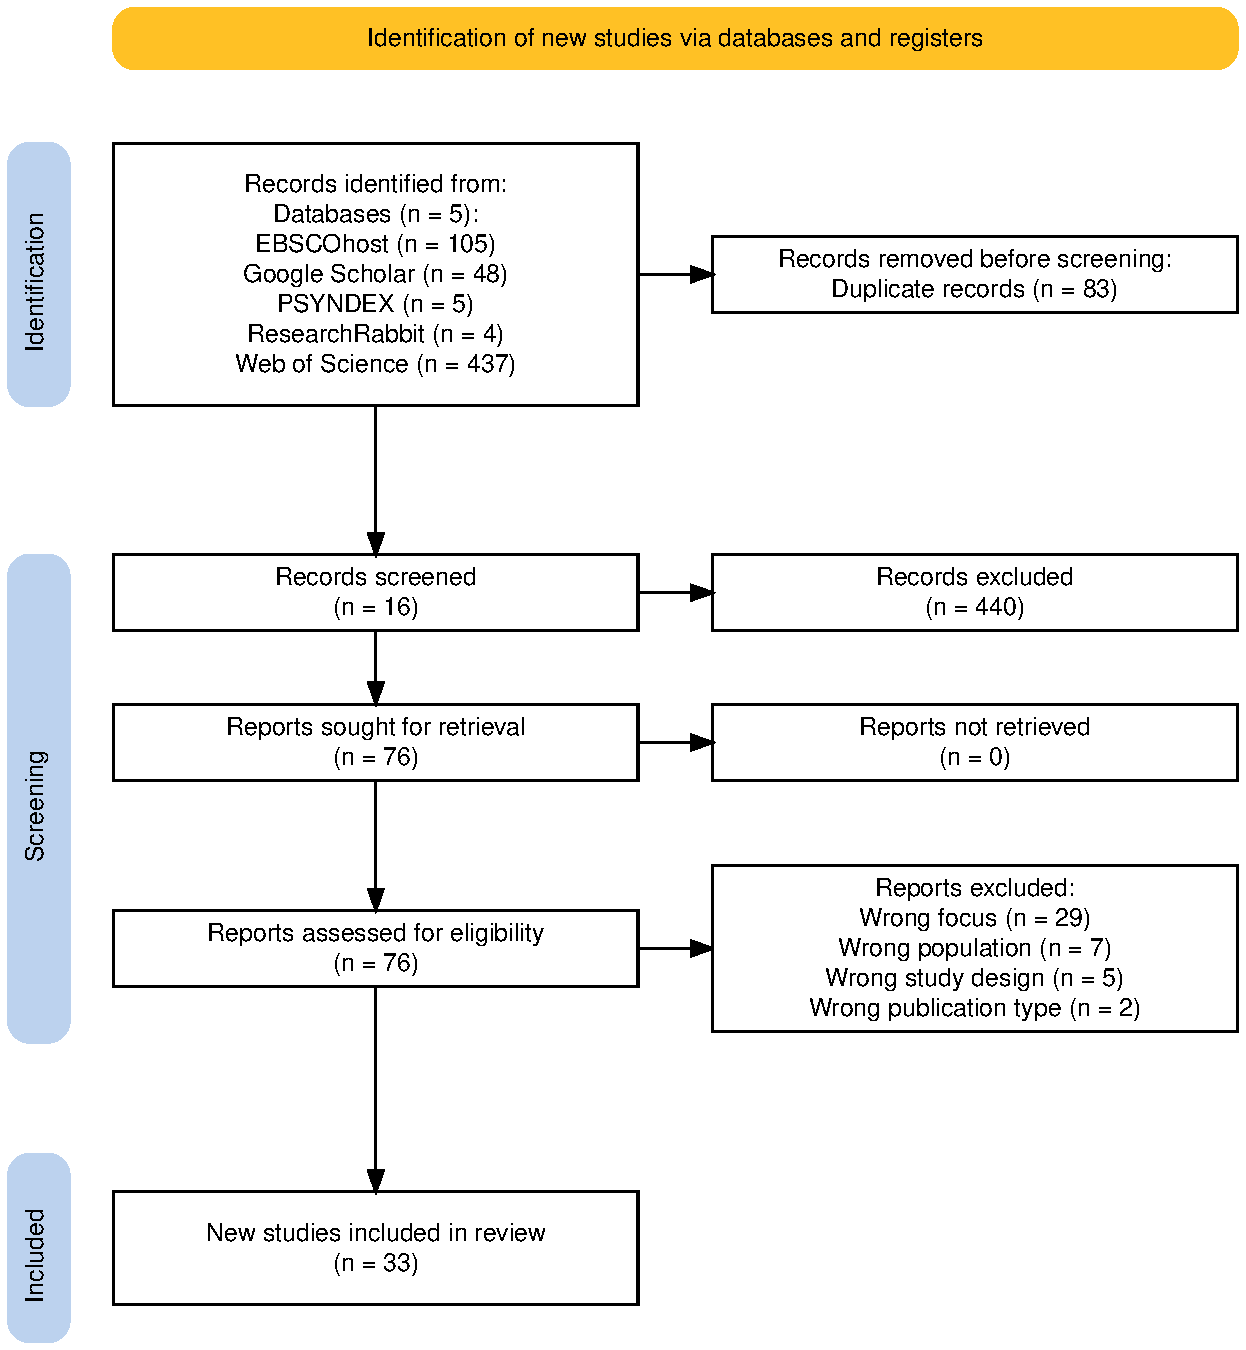
\includegraphics{files/prisma.pdf}
\caption{\label{fig:prisma}This PRISMA flow diagram illustrates the process of study selection for this systematic review. The diagram shows the number of records identified through database searching, the number of records screened and excluded, and the final number of studies included in the review. EBSCOhost, Google Scholar, PSYNDEX, ResearchRabbit, and Web of Science were the databases used for the initial search. Records were excluded based on criteria such as wrong focus, study design, population, or publication type.}
\end{figure}

\subsection{\texorpdfstring{Reporting of \emph{p}-values}{Reporting of p-values}}\label{reporting-of-p-values}

It should be noted that some \emph{p}-values are reported for example, \emph{p} \textless{} .010, this is not in accordance with APA guidelines ({``6.36 {Decimal Fractions},''} 2020); however, this format was chosen, since the papers it was taken from used this format, and it was deemed important to keep the original format, especially since it is unknown what the actual \emph{p}-value was.

\subsection{RStudio and R packages}\label{rstudio-and-r-packages}

The following R packages were used to create this review: R (Version 4.4.1; R Core Team, 2024) and the R-packages \emph{citr} (Version 0.3.2; Aust, 2019), \emph{gramr} (Version 0.0.0.9000; Dumas et al., 2024), \emph{kableExtra} (Version 1.4.0; Zhu, 2024), \emph{papaja} (Version 0.1.2.9000; Aust \& Barth, 2023), \emph{RefManageR} (Version 1.4.0; McLean, 2017), \emph{rmarkdown} (Version 2.27; Xie et al., 2018, 2020), \emph{shiny} (Version 1.8.1.1; Chang et al., 2024), and \emph{tinylabels} (Version 0.2.4; Barth, 2023).

\section{Results}\label{results}

\subsection{Hypothesis 1: Stereotype threat, brain areas/networks, performance.}\label{hypothesis-1-stereotype-threat-brain-areasnetworks-performance.}

Beilock et al. (2007) hypothesized that high-pressure situations would impair maths performance, especially under high working memory load.
The dependent variables were maths accuracy, self-reported thoughts, and reaction time (RT), while the independent variables were group (stereotype threat vs.~control), problem working demand (low vs.~high), block (baseline vs.~post-test), and \emph{2}-back task (verbal, spatial).
31 women participated in Experiment 1, 33 in Experiment 3A, and 30 in Experiment 4.
Experiment 1: Under threat, the Group \(\times\) Block \(\times\) Problem Demand interaction was found to be significant for accuracy, \emph{F}(1,29) = 11.18, \emph{p} \textless{} .010, \(\eta^{2}_{p}\) = .280.
High-demand problems, showed a significant decrease in accuracy at the post-test, CI {[}81.00\% - 97.00\%{]}; \emph{d} = 0.61.\\
Experiment 3A: For the MA problems, a three-way interaction between the independent variables was found, \emph{F}(1,31) = 4.12, \emph{p} = .050, \(\eta^{2}_{p}\) = .120.
Accuracy suffered significantly under stereotype threat; CI {[}84.00\% - 99.30\%{]}; \emph{d} = 0.64.\\
Experiment 4: A significant Block \(\times\) Problem Repetition \(\times\) Problem Working Memory demand interaction was found, \emph{F}(1, 29) = 6.13, \emph{p} \textless{} .020.
Accuracy significantly decreased under stereotype threat; CI {[}52.80\% - 77.20\%{]}; \emph{d} = 0.70) in high-demand problems.\\
Experiment 5: Under stereotype threat, an interaction between Task \(\times\) Experiment for RT, \emph{F}(1,56) = 4.38, \emph{p} \textless{} .050, \(\eta^{2}_{p}\) = .070 was found, with verbal tasks being significantly slower than spatial ones.
H1 is partially confirmed by this paper, central executive functioning is assumed to involve the prefrontal cortex; however, this is not the only area affected.
The phonological loop is associated with BA4, BA49, and (approximately) BA44 and BA45.

Dunst et al. (2013) investigated the effects of stereotype threat on neural efficiency and sex differences in visuospatial task performance, using task performance, brain activation, and neural efficiency as dependent variables, and sex, stereotype exposure, and figural intelligence as independent variables
The final sample consisted of 58 participants (\(N = 58\); 26 girls).
The TRP changes revealed a main effect for Stereotype Exposure (\emph{F}(1, 54) = 3.93, \emph{p} = .050, \(\text{partial }\eta^{2}\) = 0.07), with heightened cortical activation (\emph{M} = 0.07, \emph{SD} = 0.03) in the stereotype threat condition.
H1 is not confirmed by this paper, as the only significant effect under stereotype threat was an increase in cortical activation, which are regions of the cerebral cortex or cerebellar cortex (VandenBos \& American Psychological Association, 2015a).

In a sample of 58 participants (33 minorities), Forbes et al. (2015) investigated how DMN phase-locking at rest affects stereotype threat's impact on performance perceptions in minorities versus Whites.
Besides ethnicity (Minority vs.~White), the independent variables consisted of the phase-locking between the left lateral parietal cortex (LLPC) and precuneus/posterior cingulate cortex (P/PCC), and the phase-locking between LLPC and the medial prefrontal cortex (MPFC), each at the frequency bands alpha (8-12 Hz) and theta (4-8 Hz), these will also be referred to as DMN phase-locking, if the need to differentiate between them is not given.
Error estimates and self-doubt were used as dependent variables.\\
The relationship between LLPC-P/PCC theta phase-locking showed a main effect on error estimation (\emph{b} = -195.29, \(\beta\) = -0.37, \emph{SE} = 81.13, \emph{p} = .021), which was then moderated by a significant interaction (\emph{b} = 350.13, \(\beta\) = 0.37, \emph{SE} = 147.26, \emph{p} = .021).
Among minorities, a correlation between LLPC-MPFC theta phase-locking and self-doubt was found to be significant (\emph{r} = -0.54, \emph{p} \textless{} .010), differing significantly from Whites (\emph{z} = -2.00, \emph{p} \textless{} .050.
H1 is supported by this paper.

Forbes et al. (2008) hypothesized that error-related negativity (ERN) displays a greater amplitude under stereotype threat, and that greater Error Positivity (Pe) amplitudes to errors would be predicted under stereotype threat.\\
The study design was cross-sectional with two groups, diagnostic of intelligence (DIQ; stereotype threat) and control (no stereotype threat).
Diagnostic of intelligence (DIQ; stereotype threat) and control, alongside psychological disengagement (devaluing academics/discounting intelligence tests) were the independent variables and ERN, Pe, task performance, and self-reported measurements were the dependent variables.
The sample consisted of 57 (\(N = 57\)) minority undergraduates.
The ERN was measured as the peak negative deflection at Fz (frontal midline electrode) between 50 and 130 ms after the response, while the Pe was measured as the peak positive deflection at site Pz (midline parietal electrode) between 200 and 500 ms after the error, based on these difference waveforms.
Under stereotype threat (\(\beta\) = 0.46, \emph{p} \textless{} .010), smaller ERN amplitudes were found, with devaluing was a predictor.
On Pe amplitudes a significant moderation effect of discounting on diagnosticity was observed at Pz, \(\beta\) = 0.29, \emph{p} \textless{} .030, \(R^2\) = 0.52).
If participants were low in discounting (\(\beta_{Low}\) = -.390, \emph{p} \textless{} 0.04), smaller Pe amplitudes were found under stereotype threat.
In the opposite case, that is high discounting (\(\beta_{High}\) = 0.20, \emph{p} = .230), participants showed larger Pe amplitudes.
H1 is partially being confirmed by this paper, as neural activation was found due to stereotype threat; however, the results for the affected areas are more vague, being linked to the anterior cingulate of the prefrontal cortex.

Jończyk et al. (2022) examined the impact of stereotype threat on alpha power and creative thinking in 23 female undergraduates.
Measurements were taken before and after threat manipulation, forming the independent variables, while creative thinking (measured using Alternative Uses task; AUT, and Utopian Situations task; UST) and alpha power formed the dependent variables.
Task related power (TRP) was calculated in the lower (8-10 Hz) and upper (10-12 Hz) alpha bands before and after the stereotype threat manipulation.\\
The final sample consisted of twenty-three (\(N = 23\)) female undergraduates.\\
A main effect of threat was found in the lower alpha range (8-10 Hz), \emph{F}(1,21) = 19.41, \emph{p} \textless{} .001, \(\hat{\eta}^{2}_{G}\) = 0.05, 90\% CI {[}0.00, 0.26{]}, with greater alpha Event-Related Synchronization (ERS) after the administration of stereotype threat (\(M_{\text{post-threat}}\) = 10.00, 95\% CI {[}-4.38, 24.39{]}).
A main effect of threat was also found in the upper alpha range, \emph{F}(1, 21) = 15.42, \emph{p} \textless{} .001, \(\hat{\eta}^{2}_{G}\) = 0.05, 90\% CI {[}0.00, 0.26{]}, with greater upper alpha ERS after the administration of stereotype threat (\(M_{\text{post-threat}}\) = 3.75, 95\% CI {[}-10.09, 17.59{]}).
Comparing the upper alpha power directly before and after stereotype threat with one another, reached significance, \emph{F}(1, 21) = 15.28, \emph{p} \textless{} .001, \(\hat{\eta}^{2}_{G}\) = 0.08, 90\% CI {[}0.00, 0.31{]}, with an increase after the manipulation.
For the lower alpha power, the same comparison was significant, \emph{F}(1, 21) = 4.46, \emph{p} = .047, \(\hat{\eta}^{2}_{G}\) = 0.03, 90\% CI {[}0.00, 0.23{]}, with an increase after the manipulation.
H1 is partially supported by this paper, while stereotype threat did result in increased neural activity, the paper did not explicitly investigate stereotype effects on any of the mentioned areas. However, parts that are associated with the DMN were affected. Furthermore, performance was not found to be inhibited to a significant degree under stereotype threat.

Krendl et al. (2008) used functional magnetic resonance imaging (fMRI) to investigate underlying neural processes of stereotype threat, specifically women under maths stereotype threat.
Twenty-eight (\(N = 28\)) female undergraduates were randomly assigned to either a stereotype threat or a control condition.
Neural activation patterns and maths performance (measured by accuracy, that is, number of correct maths items; reaction time on maths problems) were used as dependent variables, stereotype threat condition (threat vs.~control) and time of measurements (Time 1: pre-manipulation vs.~Time 2: post-manipulation) functioned as independent variables.\\
For performance, a significant condition \(\times\) time interaction was found, \emph{F}(1,26) = 11.41, \emph{p} \textless{} .005, \(\eta^{2}_{p}\) = .310.
Individuals under stereotype threat performed slightly worse over time, \emph{t}(13) = 1.98, \emph{p} = .070).
No main effect of condition was found on performance.
Threatened participants did show increased vACC activation over time, \emph{t}(13) = 5.64, \emph{p} \textless{} .001, compared to controls, resulting in a significant interaction, \emph{F}(1,26) = 5.97, \emph{p} = .020.
vACC, BA11 and BA2 showed increased activation under threat, \emph{t} = 6.26, \emph{p} \textless{} .001, \emph{t}(13) = 5.63, \emph{p} \textless{} .001, and \emph{t}(13) = 5.19, \emph{p} \textless{} .001, respectively.
H1 is partially supported by this paper. It reports increases in vACC activity and decreases in BA11 (part of the PFC), along with increases in certain regions of the DMN (BA2).

Mangels et al. (2012) investigated the effects of stereotype threat on maths performance and neutral responses to feedback using three event-related potentials (ERPs): anterior P3 (P3a), medial frontal feedback-related negativity (FRN) and posteriorly-maximal late positive potential (LPP).
The study design was prospective, with sixty-eight participants (\(N = 68\)) in total.
Stereotype threat vs.~no stereotype threat formed the independent variable, maths performance (first-test vs.~retest accuracy), ERP responses to feedback, use of the tutor (number of uses and clicks when in use), and learning success (error correction on retest) were used as dependent variables.
While maths performance was impaired under stereotype threat, \emph{F}(1,64) = 4.30, \emph{p} \textless{} .050, it did not affect retest performance or error correction.
While LPP and learning success were closely linked, particularly under threat.
Participants showing greater initial detection of negative feedback (indicated by FRN differences) were more likely to disengage from tutor exploration.
Those struggling to regulate attention and arousal in response to negative feedback (indicated by LPP differences) benefited less from the tutor.
H1 is not supported, as the results of the affected areas are more vague, partially due to the ERPs not being significantly influenced by stereotype threat, and partially because it is not possible to link LPP, FRN, and P3a to the suggested brain areas/networks, if so, only to a small degree.

Wu and Zhao (2021) examined the effects of maths stereotype threat using resting-state fMRI and degree centrality (DC) analysis on 48 female Chinese undergraduates.
Significant main effects were found for the hippocampus, middle cingulate gyrus (MCG), right cerebellum, and left precentral gyrus (PCG), using a 2 (test: pre- vs post-test) \(\times\) 2 (condition: stereotype threat vs.~control) mixed-effect analysis for the binary graph.
However, out of these only MCG had increased RSDC \emph{z}-values under stereotype threat, \emph{F}(1, 45) = 4.88, \emph{p} = .032.
Further, an interaction was found to be significant between test and condition in the left cerebellum anterior lobe, left hippocampus, left precuneus, \emph{F}(1, 45) = 8.43, \emph{p} = .006, and left middle occipital gyrus (MOC).
Here, the mean RSDC \emph{z}-values were only higher in the stereotype threat condition in the right superior parietal gyrus, left precuneus, left MOG, and right angular gyrus.
The weighted graph analysis showed similar patterns, with increased RSDC z-values under threat in the middle cingulate gyrus and the aforementioned regions, except for the left cerebellum, which showed lower values.
For interactions, lower RSDC \emph{z}-values under stereotype threat were only found for the left cerebellum (F(1, 45) = 4.23, \emph{p} = .046).
H1 is partially supported by this paper, increases in the DMN (associated areas) were found as well as neural activation. However, it is unclear whether performance did suffer as a result of stereotype threat and further, while the ACC and prefrontal cortex are mentioned in the researcher's hypothesis, they are not mentioned in the results.

An overview of the included papers for Hypothesis 1 can be found in Table \ref{tab:h1_table}.

\begin{lltable}

\begin{TableNotes}[para]
\normalsize{\textit{Note.} This table presents studies examining the effects of stereotype threat on various cognitive and neural outcomes. The 'Variables' column includes both independent variables (IV) and dependent variables (DV). The 'Research Questions' column specifies the main questions investigated in each study; tasks/tests listed after the semicolon indicate which task/test was used to measure cognitive control. 'Methods of Data Analysis' specifies the statistical techniques used. 'Results' emphasize the main findings under stereotype threat conditions. Methods such as 'EEG' or 'fMRI' indicate the technique used for measurement, and the brain areas in parentheses specify which areas were found to be activated under threat. Significance levels are indicated by asterisks: *\textit{p} < .05, **\textit{p} < .01, ***\textit{p} < .001.}
\end{TableNotes}

\small{

\begin{longtable}{p{1.5cm}p{3cm}p{2.5cm}p{3cm}p{3cm}p{3cm}p{3.5cm}p{1.5cm}}\noalign{\getlongtablewidth\global\LTcapwidth=\longtablewidth}
\caption{\label{tab:h1_table}Overview of the Included Papers for Hypothesis 1}\\
\toprule
Citation & Study Design & Population & Research Questions & Variables & Methods of Data Analysis & Results & Hypothesis confirmed\\
\midrule
\endfirsthead
\caption*{\normalfont{Table \ref{tab:h1_table} continued}}\\
\toprule
Citation & Study Design & Population & Research Questions & Variables & Methods of Data Analysis & Results & Hypothesis confirmed\\
\midrule
\endhead
Beilock et al. (2007) & Experimental & Experiment 1: 31 female college students; Experiment 3A: 33 female college students; Experiment 4: 30 female college students; Experiment 5: 33 female college students & Effects of stereotype threat on working memory and its influence on unrelated tasks; behavioural tasks (phonological loop, CEN) & IV: Group (stereotype threat vs. control), Problem working memory demand (low vs. high), Block (baseline vs. posttest); DV: Accuracy, Reaction time & ANOVA & High-demand problems showed a significant decrease in accuracy at the post-test, CI [81.00\% - 97.00\%]; $\textit{d}$ = 0.61. $\textit{F}$(1,29) = 11.18**, $\eta^{2}_\text{p}$ = 0.28. & Yes\\
Dunst et al. (2013) & Experimental & 58 secondary school students in Austria & Effects of stereotype threat on neural efficiency and task performance; EEG (cerebral cortex, cerebellar cortex) & IV: Stereotype exposure; DV: Neural efficiency, Task performance & ANOVA & Heightened cortical activation ($\textit{M}$ = 0.07, $\textit{SD}$ = 0.03). $\textit{F}$(1, 54) = 3.93*, $\text{partial }\eta^{2}_\text{p}$ = 0.07. & No\\
Forbes et al. (2015) & Experimental & 58 participants (25 White, 33 minorities) & DMN phase-locking at rest and its impact on performance perceptions under stereotype threat; EEG (DMN) & IV: Phase-locking between LLPC and P/PCC, Phase-locking between LLPC and MPFC; DV: Error estimation, Self-doubt & Regression models & The relationship between LLPC-P/PCC theta phase-locking showed a main effect on error estimation and was moderated by a significant interaction. $\textit{b}$ = -195.29, $\beta$ = -0.37, $\textit{SE}$= 81.13*, $\textit{b}$ = 350.13, $\beta$ = 0.37, $\textit{SE}$ = 147.26*,). & Yes\\
Forbes et al. (2008) & Experimental & 57 minority undergraduates & Effects of stereotype threat on ERN and Pe; EEG (anterior cingulate) & IV: Diagnosticity, Psychological disengagement (devaluing academics/discounting intelligence tests); DV: ERN, Pe, Task performance, Self-reported measurements & Repeated measures analysis & Smaller ERN amplitudes were found under stereotype threat ($\beta$ = 0.46, **). A significant moderation effect of discounting on diagnosticity was observed at Pz ($\beta$ = 0.29*, $R^2$ = 0.52). & Partially\\
Jończyk et al. (2022) & Experimental & 23 female undergraduates in US & Effects of stereotype threat on alpha power and creative thinking; EEG (DMN) & IV: Threat manipulation; DV: Creative thinking, Alpha power & Repeated measures ANOVA & Greater alpha Event-Related Synchronization (ERS) was found after the administration of stereotype threat in both the lower (8-10 Hz) and upper (10-12 Hz) alpha ranges. $\textit{F}$(1,21) = 19.41***, $\hat{\eta}^{2}_\text{G}$ = 0.05, 90\% CI [0.00, 0.26]. & Partially\\
Krendl et al. (2008) & Experimental & 28 female undergraduates & Effects of stereotype threat on neural activation patterns and maths performance; fMRI (vACC, BA11, BA2) & IV: Condition (stereotype threat vs. control), Time of measurements (pre-manipulation vs. post-manipulation); DV: Neural activation patterns, Maths performance & Mixed-model ANOVA & Heightened activity in the vACC, BA11, and BA2 during the second test. $\textit{t}$ = 6.26***, $\textit{t}$(13) = 5.63***, and $\textit{t}$(13) = 5.19***, respectively & Partially\\
Mangels et al. (2012) & Prospective & 68 participants & Effects of stereotype threat on maths performance and neural responses to feedback; EEG (LPP) & IV: Stereotype threat vs. no stereotype threat; DV: Maths performance, ERP responses to feedback, Learning success & ANOVA & Maths performance was impaired under stereotype threat. $\textit{F}$(1,64) = 4.30*. & No\\
Wu and Zhao (2021) & Experimental & 48 female undergraduates in China & Effects of maths stereotype threat on brain region connectivity; rs-fMRI (left precuneous, hippocampus, MCG, cerebellum) & IV: Test (pre- vs post-test), Condition (stereotype threat vs. control); DV: RSDC of brain regions & Mixed-effect analysis & Significant main effects were found for the hippocampus, MCG, right cerebellum, and left PCG; left precuneus: $\textit{F}$(1,45) = 8.43**. & Partially\\
\bottomrule
\addlinespace
\insertTableNotes
\end{longtable}

}

\end{lltable}

\subsection{Hypothesis 2: Stereotype threat, cognitive control.}\label{hypothesis-2-stereotype-threat-cognitive-control.}

Guardabassi and Tomasetto (2020) hypothesized that BMI and working memory were negatively, whether this effect was increased by stereotype threat, and whether this effect can be moderated by endorsement.
Body Mass Index (BMI), stereotype threat condition (threat vs.~control), personal endorsement of obesity-related stereotypes (stereotype endorsement), and weight-based teasing, as independent variables, working memory performance (\emph{N}-back task performance; 0-back up to two-back) was used as the dependent variable.
The final sample consisted of 176 primary school children, 106 of which were boys (\(M_{\text{age}}\) = 116.07 months, \emph{SD} = 10.43).
A significant main effect was found for \emph{N}-back difficulty, F(2, 198.70) = 43.43, \emph{p} \textless{} .001, and the condition \(\times\) \emph{z}BMI interaction, F(1, 153.07) = 5.07, \emph{p} = .026.
Under stereotype threat, \emph{z}BMI scores negatively correlated with working memory.
H2 is weakly supported by this paper, while stereotype threat did decrease \emph{N}-back task performance, it cannot be divided which parts of working memory were affected, since the \emph{N}-back task does involve multiple parts of working memory.

Hirnstein et al. (2014) investigated the effects of stereotype threat on sex differences in cognitive performance and its relation to testosterone levels.
A final sample of 136 participants (\(n_{\text{female}} = 70\)) were tested in a 2 (stereotype threat vs.~control) \(\times\) 2 (mixed vs.~same sex) \(\times\) 2 (male vs.~female) factorial design, which formed the independent variables.
Cognitive performance (tested using mental rotation, verbal fluency, and perceptual speed tests) alongside testosterone levels, were used as dependent variables.
The MRT-3D showed a significant main effect of Sex, with men performing better than women, \emph{F}(1,128) = 10.97, \emph{p} = .001, \(\eta^{2}\) = 0.08, \emph{d} = 0.57, while Condition showed a significant main effect in the MP-2D, \emph{F}(1,128) = 4.70, \emph{p} = .032, \(\eta^{2}\) = 0.04.
For verbal fluency, interactions were found between Condition and Group Sex Composition, in both, the WF, \emph{F}(1,128) = 4.49, \emph{p} = .036, \(\eta^{2}\) = 0.03,and the 4W, \emph{F}(1,128) = 6.30, \emph{p} = .013, \(\eta^{2}\) = 0.05).
Between Sex \(\times\) Condition, another interaction was found, in the 4W, \emph{F}(1,128) = 6.77, \emph{p} = .011, \(\eta^{2}\) = 0.05.
Furthermore, in the 4W, Condition showed a significant main effect, \emph{F}(1,128) = 4.67, \emph{p} = .033, \(\eta^{2}\) = 0.04.
PS also showed the significant Condition and Group Sex Composition interaction, \emph{F}(1,128) = 6.89, \emph{p} = .009, \(\eta^{2}\) = 0.05.
Condition, again showed a significant main effect, this time in the PS, \emph{F}(1,128) = 12.65, \emph{p} = .001, \(\eta^{2}\) = 0.09.
H2 is weakly but partially being supported, since individuals under stereotype threat performed worse on the 4W (but not WF) and perceptual speed tests, which measure cognitive control among other things.

In this study, the Jordano and Touron (2017b) investigated the effects of stereotype threat on both, cognitive performance and task-related mind-wandering.
In both experiments sixty female undergraduates were assigned to either a stereotype threat or control condition; mind-wandering --- measured using Task-Unrelated Thoughts (TUTs) and Task-Related Inference (TRI) probes ---, task performance (on the Operation Span task; OSPAN), and self-reported measures (i.e., emotional states, cognitive load/perceived difficulty, experience of mind-wandering), were used as dependent variables.
In the first experiment, it was found that participants under stereotype threat reported significantly more TRI compared to the control group, \emph{F}(1,58) = 5.67, \emph{p} = .021, \emph{d} = 0.64.\\
Neither maths verification accuracy nor letter recall accuracy were worse under stereotype threat.
In the second experiment, the same pattern was found, with participants under stereotype threat reporting significantly more TRI, \emph{F}(1,58) = 5.53, \emph{p} = .022, \emph{d} = 0.42.
Maths verification accuracy was worse under stereotype threat, \emph{F}(1,58) = 12.11, \emph{p} = .001, \emph{d} = 0.16.
H2 is partially confirmed. While cognitive control did suffer under stereotype threat, as evidenced by increased mind-wandering (TRI), regardless of task difficulty, task performance only worsened in the more difficult maths component of the OSPAN task.

Krendl et al. (2008) has already been reported in the H1 section.
H2 is supported, due to decreased accuracy under stereotype threat, as well as neural activation patterns (vACC).

Lin et al. (2023) investigated the mediating role of executive function in stereotype threat effects on spatial perspective-taking tasks.
Stereotype threat (threat vs.~control) served as the independent variable, while spatial perspective-taking performance and executive function performance (inhibition, updating, shifting) were used as dependent variables.
Seventy-six undergraduates participated
A significant decrease in performance was found for the threat group, \emph{F}(1,74) = 10.06, \emph{p} = .002, \(\eta^{2}\) = 0.12).\\
In Experiment 2, seventy-seven undergraduates participated.\\
The effect of stereotype threat was significant for inhibition and updating, \emph{F}(1,75) = 11.40, \emph{p} = .001, \(\eta^{2}\) = 0.13), and \emph{F}(1,75) = 5.54, \emph{p} = .021, \(\eta^{2}\) = 0.07), respectively.
Females under threat performed worse on the spatial perspective-taking task.
Only inhibition showed a significant (indirect) mediating effect.
Further, between spatial perspective-taking and stereotype threat, a significant direct effect was found, \(\text{direct effect}\) = 0.38, \emph{SE} = 0.18, \emph{t} = 2.06 95\% \(\text{CI}\) {[}0.01, 0.75{]}, also, significant negative effects of stereotype threat on inhibition (\emph{b} = -0.73, \emph{SE} = 0.22, \emph{t} = -3.38 CI {[}-1.51, -0.30{]}) and updating (\emph{b} = -0.52, \emph{SE} = 0.22, \emph{t} = -2.35, 95\% CI {[}-0.96, -0.08{]}) were found.
H2 is partially supported by this paper, as cognitive control (updating and inhibition) and performance did suffer under stereotype threat; however, shifting did not reach significance.

Rydell et al. (2014) examined the effects of stereotype threat on executive functions and maths performance across three experiments.
The independent variable was condition (stereotype threat vs.~control), while maths performance, executive function (inhibition, updating, shifting), and risk-taking behaviour functioned as dependent variables.
In the first experiment, 168 (\(n_{\text{female}}\) = 75) undergraduates participated.
Stereotype threat significantly impaired women's inhibition, \emph{F}(1,164) = 7.95, \emph{p} = .005, \(\eta^{2}_{\text{p}}\) = .046) and updating, \emph{F}(1,164) = 20.89, \emph{p} \textless{} .001, \(\eta^{2}_{\text{p}}\) = .113.
A performance decrease under threat was found, for accuracy, \emph{F}(1,164) = 20.22, \emph{p} \textless{} .001, \(\eta^{2}_{\text{p}}\) = .110.\\
Experiment 2 used a sample of ninety female undergraduates.
Regarding maths performance, under threat, accuracy, \emph{t}(88) = -3.15, \emph{p} = .002, \emph{d} = -0.66 and the correct item count, \emph{t}(88) = -5.15, \emph{p} \textless{} .001, \emph{d} = -1.09 were impaired, with updating mediating this effect.\\
In Experiment 3, a sample of eighty-two female undergraduates participated.
Inhibition, \emph{t}(79) = -2.34, \emph{p} = .020, \emph{d} = -0.50, and updating, \emph{t}(79) = -2.29, \emph{p} = .030, \emph{d} = -0.50, were significantly affected by stereotype threat
The results for maths performance, showed accuracy, \emph{t}(79) = -3.28, \emph{p} = .010, \emph{d} = -0.70, and the correct item count, \emph{t}(79) = -2.14, \emph{p} = .035, \emph{d} = -0.48 being impaired.
Under threat, women were more likely to take risks; however, no correlation between it and maths performance was found.
The paper more so supports H2 than it does not. Shifting repeatedly did not reach significance, while the other executive functions did.

Ståhl et al. (2012) investigated the role of regulatory focus in stereotype threat effects on cognitive control and maths performance across three experiments.
The study used varying combinations of independent variables: condition (stereotype threat vs.~no threat), regulatory focus (prevention focus vs.~promotion focus vs.~no focus), and task order (maths task first vs.~maths task last).
Dependent variables were cognitive control capacity (measured by a Stroop task) and maths performance (accuracy and response time on an MA task).
Sixty-three social science students (\(n_{\text{female}}\) = 50) participated in Experiment 1, one hundred eight social science students (\(n_{\text{female}}\) = 82, \(n_{\text{male}}\) = 26) in Experiment 2, and one hundred sixty-four female students in Experiment 3.
A significant effect of stereotype threat on Stroop inference was found, \emph{F}(1,61) = 8.69, \emph{p} = .004, \(\eta^{2}_{\text{p}}\) = .130.
Experiment 2 found a main effect of threat, \emph{F}(1,102) = 8.91, \emph{p} = .004, \(\eta^{2}_{\text{p}}\) = .080.
Further, Experiment 1's results for the Stroop task, were replicated, \emph{F}(1, 101) = 2.80, \emph{p} \textless{} 0.10, \(\eta^{2}_{\text{p}}\) = .030, and an interaction on Stroop inferences were found, \emph{F}(2,101) = 3.07, \emph{p} = .050, \(\eta^{2}_{\text{p}}\) = .060).
The Stroop inference was only significant under threat, in the prevention condition, \emph{F}(1,101) = 3.60, \emph{p} = .240, \(\eta^{2}_{\text{p}}\) = .010.\\
In Experiment 3, an interaction was found to be significant on maths performance (\% of correct responses), \emph{F}(1,150) = 13.30, \emph{p} \textless{} .001, \(\eta^{2}_{\text{p}}\) = .080.
Furthermore, only in the prevention focus condition, when the maths task came first, individuals under threat were found to perform better.
For maths performance, measured as RT, the same three-way interaction was significant, \emph{F}(1,152) = 4.69, \emph{p} = .030, \(\eta^{2}_{\text{p}}\) = .030.
For the maths first condition, prevention focus results in better performance under threat.
In the maths last condition, the two-way interaction was marginally significant.
H2 is mostly supported by this paper, albeit, only under prevention focus - and here also only after the initial temporary increase in cognitive control (Experiment 3).

Wister et al. (2013) hypothesized that menstruation stereotype threat would impair performance on cognitive tasks, this effect would be amplified if women believed menstruation to be a hindrance to their cognitive abilities.
However, if menstruation was primed as a positive influence, cognitive performance would not be impaired.
Ninety-two female undergraduates were assigned into four groups, 2 stereotype threat (menstruation threat vs.~no threat) \(\times\) 2 menstruation prime (positive vs.~no positive prime), forming the independent variables, while cognitive performance (measured by a Stroop test and SAT-like maths test) and menstrual attitudes (measured by Menstrual Attitude Questionnaire; MAQ) were used as dependent variables.
The experiment ended for everyone with the completion of the Menstrual Attitudes Questionnaire.\\
While a main effect of threat on Stroop performance was found, Lambda = 0.87, \emph{F}(1,68) = 4.91, \emph{p} \textless{} .010.
Participants under threat were able to complete less items correctly, \emph{F}(1,69) = 9.48, \emph{p} \textless{} 0.01, and a correlation between closeness to menstruation and both, Stroop performance, \emph{r} = -0.56, \emph{p} = .011, and positive prime effectiveness, \emph{r} = -0.46, \emph{p} = .610 were found, with individuals in the Menstruation Threat/Positive Prime condition performing worst.
H2 is partially supported by this paper, cognitive performance under threat did only suffer if measured on the Stroop task, further, the prime also influenced performance.

Wulandari and Hendrawan (2020) hypothesized that how gender-stereotype threat is being activated, affects performance differently, depending on gender and task difficulty.
Participants were assigned to one of four groups, differing in the gender-stereotype threat activation (blatant vs.~moderately explicit vs.~subtle vs.~control), forming the independent variables, alongside gender (male vs.~female) and task difficulty (easy vs.~medium vs.~hard), while letter fluency performance (number of correct words/errors) and cognitive processes (clusterings/switching) were used as dependent variables.
The sample consisted of 168 undergraduates (\(n_{\text{female}}\) = 91).\\
No significant effect was found for switching, neither for gender, nor for threat; for cluster size, only a significant effect of gender was found, \emph{F}(1,159) = 4.12, \emph{p} \textless{} .050, \(\eta^{2}_{\text{p}}\) = .025, with males scoring higher than females.
Also, positive correlations between total errors and gender-stereotype score, \emph{r} = 0.22, \emph{p} \textless{} .010, were found, with gender-stereotype scores being the result of the gender-stereotype questionnaire.
H2 is not supported by this paper, more so, it provides evidence against it.

An overview of the included papers for Hypothesis 2 can be found in Table \ref{tab:h2_table}.

\begin{lltable}

\begin{TableNotes}[para]
\normalsize{\textit{Note.} This table presents studies examining cognitive control processes under stereotype threat. The 'Variables' column includes both independent variables (IV) and dependent variables (DV). 'Methods of Data Analysis' specifies the statistical techniques used. Tasks/tests listed after the semicolon in the Research Questions column indicate which task/test was used to measure cognitive control. 'Results' emphasize changes in cognitive control performance under stereotype threat conditions, with significance levels indicated by asterisks: *\textit{p} < .05, **\textit{p} < .01, ***\textit{p} < .001.}
\end{TableNotes}

\small{

\begin{longtable}{p{1.8cm}p{2.6cm}p{2.5cm}p{3cm}p{3cm}p{3cm}p{3.5cm}p{1.5cm}}\noalign{\getlongtablewidth\global\LTcapwidth=\longtablewidth}
\caption{\label{tab:h2_table}Overview of the Included Papers for Hypothesis 2}\\
\toprule
Citation & Study Design & Population & Research Questions & Variables & Methods of Data Analysis & Results & Hypothesis confirmed\\
\midrule
\endfirsthead
\caption*{\normalfont{Table \ref{tab:h2_table} continued}}\\
\toprule
Citation & Study Design & Population & Research Questions & Variables & Methods of Data Analysis & Results & Hypothesis confirmed\\
\midrule
\endhead
Guardabassi and Tomasetto (2020) & Cross-sectional & 176 primary school children & Effects of weight stereotype threat on working memory; N-back task & IV: BMI, Stereotype threat; DV: Working memory & Mixed-effects models & Under stereotype threat, zBMI scores negatively correlated with working memory; $\textit{F}$(2, 198.70) = 43.43***, $\textit{F}$(1, 153.07) = 5.07* & Partially\\
Hirnstein et al. (2014) & Factorial & 136 participants (66 male, 70 female) & Effects of stereotype threat, sex, and group composition on cognitive performance; Cognitive tests & IV: Stereotype threat, Sex, Group composition; DV: Cognitive performance & ANOVA & Performance decreased on 4W and perceptual speed under threat; $\textit{F}$(1,128) = 6.30*, $\eta^{2}_\text{p}$ = .050 & Weakly\\
Jordano and Touron (2017) & Experimental & 120 female undergraduates & Effects of stereotype threat on mind-wandering and task performance; OSPAN task, mind-wandering probes & IV: Stereotype threat; DV: Mind-wandering, Task performance & ANOVA & Increased mind-wandering, decreased maths performance under threat; $\textit{F}$(1,58) = 12.11***, $\eta^{2}_\text{p}$ = .164 & Partially\\
Krendl et al. (2008) & Experimental & 28 female undergraduates & Effects of stereotype threat on neural activation and maths performance; fMRI (vACC, BA11, BA2) & IV: Condition (stereotype threat vs. control), Time of measurements; DV: Neural activation patterns, Maths performance & Mixed-model ANOVA & Heightened activity in the vACC, BA11, and BA2 during the second test. $\textit{t}$ = 6.26***, $\textit{t}$(13) = 5.63***, and $\textit{t}$(13) = 5.19***, respectively & Yes\\
Lin et al. (2023) & Cross-sectional & 153 female undergraduates & Effects of stereotype threat on spatial performance and executive function; Spatial perspective-taking, executive function tests & IV: Stereotype threat; DV: Spatial performance, Executive function & ANCOVA, mediation analysis & Decreased performance, impaired inhibition and updating under threat; $\textit{F}$(1,74) = 10.06**, $\eta^{2}_\text{p}$ = .120 & Partially\\
Rydell et al. (2014) & Experimental & 340 undergraduates across 3 experiments & Effects of stereotype threat on executive function and maths performance; Executive function tasks, maths tests & IV: Stereotype threat; DV: Executive function, Maths performance & ANOVA, mediation analysis & Impaired inhibition and updating, decreased maths performance under threat; $\textit{F}$(1,164) = 20.22***, $\eta^{2}_\text{p}$ = .110 & Mostly\\
Ståhl et al. (2012) & Experimental & 335 students across 3 experiments & Effects of stereotype threat and regulatory focus on cognitive control; Stroop task, maths task & IV: Stereotype threat, Regulatory focus; DV: Cognitive control, Maths performance & ANOVA & Initial increase then decrease in cognitive control under threat (prevention focus); $\textit{F}$(1,150) = 13.30***, $\eta^{2}_\text{p}$ = .080 & Mostly\\
Wister et al. (2013) & Experimental & 92 female undergraduates & Effects of menstruation stereotype threat on cognitive performance; Stroop test, SAT-like maths test & IV: Menstruation threat, Positive prime; DV: Cognitive performance & MANOVA & Impaired Stroop performance under menstruation threat; $\textit{F}$(1,68) = 4.91**, $\eta^{2}_\text{p}$ = .130 & Partially\\
Wulandari and Hendrawan (2020) & Experimental & 168 undergraduates (91 female) & Effects of stereotype threat activation on task performance; Letter fluency test & IV: Stereotype threat activation, Gender, Task difficulty; DV: Task performance & ANOVA & No significant effects of threat on performance; $\textit{F}$(1,159) = 4.12*, $\eta^{2}_\text{p}$ = .025 & No\\
\bottomrule
\addlinespace
\insertTableNotes
\end{longtable}

}

\end{lltable}

\subsection{Hypothesis 3: Stereotype threat, working memory.}\label{hypothesis-3-stereotype-threat-working-memory.}

Bedyńska et al. (2020) investigated the relationships between chronic stereotype threat, language achievement, and domain identification in a sample of 319 male secondary school students.
The study utilized chronic stereotype threat as the independent variable, while language achievement and domain identification served as dependent variables. Additionally, working memory and intellectual helplessness were examined as mediators, and gender identification was explored as a moderator.
The researchers found an overall moderate level of stereotype threat in the sample, with only a slight correlation between stereotype threat and both intellectual helplessness and working memory (\emph{r} = 0.32).
Stereotype threat did negatively impact working memory capacity, with the latter mediating the relationship between stereotype threat and language achievement, \emph{b} = 2.81, \(\beta\) = 0.45, \emph{SE} = 0.06, \emph{p} \textless{} .001, 95\% CI {[}0.34, 0.55{]}.
Language achievement was indirectly affected by stereotype threat, through impaired working memory and intellectual helplessness.
H3 is supported by this paper; however it should be noted that it was chronic stereotype threat that was investigated and that the level of threat was only moderate.

Bedyńska et al. (2018) examined the effects of chronic stereotype threat on mathematical achievement in a sample of 624 female secondary school students.
The study employed chronic stereotype threat as the independent variable and mathematical achievement as the dependent variable, with working memory and intellectual helplessness serving as mediators and gender identification as a moderator.
The researchers found a slight correlation between stereotype threat and intellectual helplessness (\emph{r} = 0.20),while maths achievement showed significant correlations with working memory (\emph{p} \textless{} .010), and both stereotype threat and intellectual helplessness (\emph{p} \textless{} .010), with the former being positive and the latter negative.
Working memory was negatively impacted by chronic stereotype threat, \emph{b} = -0.01, \(\beta\) = -0.11, \emph{SE} = 0.13, \emph{p} = .378, albeit not significantly.
Gender identity did moderate the effect of stereotype threat on working memory, amplifying the negative effect, \emph{b} = -0.01, \(\beta\) = -0.29, \emph{SE} = 0.14, \emph{p} = .039.
H3 is supported by this paper; however, it needs to be noted that it was chronic stereotype threat that was investigated.

Beilock et al. (2007) was already discussed in the H1 section.
H3 is supported by this paper, clear impairments on maths performance are found.

Brown and Harkins (2016) investigated the effects of stereotype threat on mind-wandering in 73 female undergraduates, using the Sustained Attention to Response Task (SART).
The study employed a 2 \(\times\) 2 design with condition (stereotype threat vs.~control) and SART framing (related to maths ability vs.~unrelated to maths ability) as independent variables, and mind-wandering (measured by SART performance) as the dependent variable. The researchers hypothesized that participants under threat would show more mind-wandering, unless the SART was framed as related to maths ability, in which case they would show less mind-wandering due to increased motivation and effort.
Both manipulations were successful.
In the Stereotype Threat/SART Related condition, commission errors were fewer (\emph{M} = 4.89, \emph{SD} = 3.03), compared to Stereotype Threat/SART Unrelated (\emph{M} = 10.44, \emph{SD} = 4.55), \emph{F}(1, 69) = 28.78, \emph{p} \textless{} .001, \(\eta^{2}_{\text{p}}\) 0.29, anticipations were lower in the Stereotype Threat/SART Related condition (\emph{M} = 0.56, \emph{SD} = 1.10), compared to Stereotype Threat/SART Unrelated (\emph{M} = 4.44, \emph{SD} = 7.09), \emph{F}(1, 69) = 11.42, \emph{p} \textless{} .010, \(\eta^{2}_{\text{p}}\) = .142, and RT coefficient of variation showed less variability in the Stereotype Threat/SART Related condition (\emph{M} = 258.00, \emph{SD} = 76.00), compared to Stereotype Threat/SART Unrelated (\emph{M} = 341.00, \emph{SD} = 97.00), \emph{F}(1, 69) = 11.75, \emph{p} \textless{} .001, \(\eta^{2}_{\text{p}}\) = .146.
H3 is not supported by this paper, as the mere effort account was found to be the more likely explanation for the results.

Guardabassi and Tomasetto (2020) was already discussed in the H2 section.
H3 is supported by this paper, as \emph{N}-back task performance was found to be impaired under stereotype threat.

Hutchison et al. (2013) examined the effects of stereotype threat on mind-wandering and Stroop task performance in a sample of 187 men (88.5\% Caucasian). The study used working memory capacity (measured by OSPAN), list congruency (mostly congruent vs.~mostly incongruent), and stereotype threat condition (threat vs.~control) as independent variables, while Stroop task performance (error rates and reaction times) served as the dependent variable. The researchers hypothesized that mind-wandering would increase under threat, impairing Stroop task performance, particularly in incongruent trials.
While the two-way interaction between stereotype threat and working memory capacity was moderate, \(\beta\) = -0.11, \emph{t} = -1.93, \emph{p} = .054, a main effect was found for stereotype threat, \(\beta\) = .120, \emph{t} = 2.11, \emph{p} \textless{} .050, showing the Stroop effect to be larger under threat.
Further, the interaction with list congruency was found to qualify this main effect, with mostly congruent lists, \(\beta\) = .240, \emph{t} = 2.55, \emph{p} \textless{} .050, showing a greater Stroop effect under threat, than mostly incongruent lists, \(\beta\) = -0.02, \emph{t} = -0.17, \emph{p} = .860,
Building on this, the interaction between all independent variables was found to be significant, \(\beta\) = -0.12, \emph{t} = -1.99, \emph{p} \textless{} .050.
Reaction times on the Stroop task were also decreased under threat to a significant degree, \(R^2\) = .530, \emph{F}(7, 174) = 28.95, \emph{p} \textless{} .001.\\
H3 is partially supported, a significant effect of threat on Stroop performance was only found for low working memory capacity individuals.
Further, working memory capacity might moderate the effect.

Jamieson and Harkins (2007) investigated the effects of stereotype threat on tasks requiring inhibitory control across four experiments.
The study used condition (stereotype threat vs.~control), task type (anti-saccade vs.~pro-saccade), and cognitive load (2-back vs.~0-back task) as independent variables, while accuracy, reaction time (RT), and eye movements served as dependent variables.
Experiment 1 displayed the target in the saccade task for 150 ms, Experiment 2, 3, and 4 for 250 ms.
In Experiment 1 the sample consisted of eighty undergraduates, Experiments 2 and 3 had thirty-six female undergraduates, and Experiment 4 seventy-two.
Performance on the anti-saccade task was impaired for participants under threat, compared to controls, \emph{F}(1, 72) = 17.28, \emph{p} \textless{} .001, \emph{d} = 0.98.
The interaction between Condition \(\times\) Task indicated that under threat, response times were lower, to a significant degree, \emph{F}(1, 72) = 4.85, \emph{p} = .050, further, under threat, accuracy was also higher for the anti-saccade trails, \emph{F}(1, 32) = 9.06, \emph{p} = .010, \emph{d} = 1.06, while it was lower for pro-saccade trails, \emph{F}(1, 32) = 8.30, \emph{p} = .010, \emph{d} = 1.01.\\
In Experiment 2, RTs were, again, faster under threat in both saccade tasks, \emph{F}(1, 32) = 19.52, \emph{p} \textless{} .001, \emph{d} = 1.58).
In Experiment 3, RT was lower in the stereotype threat condition, \emph{F}(1, 32) = 30.74, \emph{p} \textless{} .001, \emph{d} = 1.96.
Further, contrasts showed that this was true for both the anti- and pro-saccade tasks, \emph{F}(1, 32) = 29.53, \emph{p} \textless{} .001, \emph{d} = 1.91 and \emph{F}(1, 32) = 43.47, \emph{p} \textless{} .001, \emph{d} = 2.34, respectively - the same can be said for the adjusted reaction times from the eye movements, \emph{F}(1, 31) = 10.06, \emph{p} = .010, \emph{d} = 1.12.\\
In Experiment 4, \emph{n}-back task performance did not differ between controls and participants under threat, neither did accuracy.
Previous results for reaction time under threat were only replicated for the 0-back condition, \emph{F}(1, 64) = 13.67, \emph{p} = .010, \emph{d} = 0.93, while the 2-back condition showed a reduction in speed for participants under threat, \emph{F}(1, 64) = 12.15, \emph{p} = .010, \emph{d} = 0.87.
H3 is mostly not supported by this paper, only the slower reaction times under high cognitive load indicate decrease working memory speed (it is not a direct measure of working memory speed), while the other results rather support the mere effort account, which is an alternative hypothesis to the working memory account.

Johns et al. (2008) conducted a series of experiments to examine the effects of stereotype threat on working memory capacity, attention allocation to anxiety-related stimuli, and maths performance.
The study used condition (stereotype threat vs.~control), emotion regulation strategy, anxiety measure description, and ethnicity as independent variables, while working memory capacity, attention allocation, maths performance, and self-reported anxiety served as dependent variables.
In Experiment 1, eighty-one Caucasian female students participated
In the working memory task, women were able to recall fewer words under threat, resulting in a main effect of threat, \emph{F}(1, 77) = 9.53, \emph{p} \textless{} .010.
A significant Condition \(\times\) Anxiety measure description interaction was found for attention allocation, \emph{F}(1, 77) = 6.41, \emph{p} = .010, with more attention given to anxiety-related stimuli under threat when the task was framed as a measure of perceptual focus.
Experiment 3 had sixty-one Caucasian women participating.
Working memory performance did suffer under stereotype threat; however, just in the threat only condition, \emph{t}(55) = 2.31, \emph{p} \textless{} .050, \emph{d} = 0.62, the same results were found for maths test performance, \emph{t}(55) = 2.11, \emph{p} \textless{} .050, \emph{d} = 0.64.
Working memory performance was found to mediate the relationship between stereotype threat and maths performance, \(\beta\) = .300, \emph{p} \textless{} .050.
In Experiment 4, thirty-four Latino (22 women) and forty-seven Caucasians (28 women) participated.
In the threat only condition, anxiety-related words received less attention by Latinos, \emph{t}(71) = 2.47, \emph{p} \textless{} .050, \emph{d} = 0.70.
Working memory performance was significantly impaired for Latinos under only stereotype threat, \emph{t}(71) = 2.18, \emph{p} \textless{} .050, \emph{d} = 0.55.
Further, Caucasians in the threat only condition recalled the most words, while Latinos and Caucasians did not significantly differ in performance in the anxiety reappraisal condition.
H3 is supported by this paper.

Pennington et al. (2019) conducted two experiments to investigate the effects of positive and negative stereotypes on cognitive performance.
The study used stereotype condition as the independent variable, with levels varying between experiments.
Experiment 1 used self-as-target stereotype threat, group-as-target stereotype threat, and no-threat control, while Experiment 2 employed negative/positive group-as-target stereotype threat and non-threat control.
The dependent variables included anti-saccade task performance measures and, in Experiment 2, maths task performance.
In Experiment 1, participants were sixty-four female undergraduates.
One of the manipulation checks was significant, while the other was not.
For the anti-saccade task, neither SRT for correct saccades, nor their accuracy revealed a significant main effect of stereotype threat, \emph{F}(2, 58) = 0.30, \emph{p} = .750, \(\eta^{2}_{\text{p}}\) = .010), and \emph{F}(2, 57) = 0.03, \emph{p} = .970, \(\eta^{2}_{\text{p}}\) \textless{} .001, respectively.
The same can be said for reflexive saccades and their SRTs, \emph{F}(2, 57) = 0.03, \emph{p} = .970, \(\eta^{2}_{\text{p}}\) \textless{} .001, and \emph{F}(2, 56) = 0.25, \emph{p} = .780, \(\eta^{2}_{\text{p}}\) = .009, respectively.
While the SRTs for corrective saccades, again, did not reach significance for stereotype threat, \emph{F}(2, 53) = 0.30, \emph{p} = .750, \(\eta^{2}_{\text{p}}\) = .010, the percentage of corrective saccades did, \emph{F}(2, 57) = 3.57, \emph{p} = .004, \(\eta^{2}_{\text{p}}\) = .110.\\
The sample in Experiment 2 consisted of sixty female undergraduates.
The manipulation checks were successful.
On the anti-saccade task, no significant main effects were found for any of the performance measures, the same can be said for the MA task.
This paper does not support H3. In Experiment 1 there is weak evidence of a few impairments; however, overall stereotype threat did not seem to significantly alter performance.

Rydell et al. (2009) hypothesized that different social identities can mitigate the performance impairments of stereotype threat.
Further, a positive social identity can lighten the depletion of working memory capacity under stereotype threat.\\
Gender stereotype (present vs.~absent) and college student stereotype (present vs.~absent) were the independent variables, while working memory capacity alongside maths performance and vowel counting accuracy were the dependent variables.
Fifty-seven (\(N = 57\)) female undergraduates participated in the study.
A significant two-way interaction was found between both stereotype conditions, \emph{F}(1, 53) = 6.01, \emph{p} = .020, \(\eta^{2}_{\text{p}}\) = .102, without gender-stereotypes, performance did not differ between the college student stereotype conditions.
Further, under gender-stereotype threat, maths performance did suffer to a significant degree.
Working memory showed the same pattern, with, the two-way interaction being significant, \emph{F}(1, 53) = 4.91, \emph{p} = .030, \(\eta^{2}_{\text{p}}\) = .080, the without gender stereotypes conditions showing no significant differences, \emph{F}(1, 27) = 2.33, \emph{p} = .140, \(\eta^{2}_{\text{p}}\) = .008.
The number of words recalled was lower, for those under gender-stereotype threat, who did not have the college student stereotype, \emph{F}(1, 26) = 31.41, \emph{p} \textless{} .001, \(\eta^{2}_{\text{p}}\) = .547.
Working memory capacity mediated the relationship of both stereotypes and maths performance, as analysed with a Sobel test, \emph{z} = 1.96, \emph{p} = .050.
H3 is supported by this paper.

Schmader et al. (2009) conducted two experiments to examine the relationship between anxiety, stereotype threat, and working memory capacity.
The study used prime condition (confidence vs.~doubt) and self-reported anxiety as independent variables in both experiments, with additional variables of ethnicity in Experiment 1 and task frame in Experiment 2.
Working memory performance, measured by a modified Reading Span Test, served as the dependent variable.
The final sample in Experiment 1 consisted of 37 minorities (17 Hispanics, 16 African Americans, and 4 American Indian) and 40 Whites (\(N = 77\)).
While the Prime \(\times\) Ethnicity interaction did not reveal a main effect on anxiety, a marginal one was found for ethnicity, \emph{F}(1, 73) = 2.92, \emph{p} = .090.
For working memory, the sentence reading times did not differ significantly between conditions.\\
In Experiment 2, the final sample consisted of 111 females (79 White, 10 Hispanic, 7 African American, 7 Asian American, 1 American Indian, and 7 unidentified; \(N = 111\)).\\
A prime \(\times\) task frame interaction was found for anxiety, \emph{F}(1, 107) = 3.83, \emph{p} = .050, with anxiety being higher in the maths test condition, compared to the problem-solving task; however, significance was not reached, while also not reaching significance, the opposite pattern was found for women in the confidence condition.
For working memory the three-way interaction among task frame, prime, and anxiety level was significant, \(\beta\) = -0.20, \emph{p} = .050.
If the task was framed to be diagnostic (stereotype threat), the anxiety \(\times\) prime interaction was significant, \(\beta\) = -0.30, \emph{p} \textless{} .040, with higher anxiety and doubt resulting in significantly lower working memory performance, while lower anxiety showed no effects, independently of the prime.
H3 is partially supported by this paper, as Study 1 does not support it, while Study 2 does.

Schmader and Johns (2003) conducted three experiments to investigate the effects of stereotype threat on working memory capacity and maths test performance.
The study used condition (stereotype threat vs.~control) as an independent variable across all experiments, with additional variables of gender in Experiment 1 and ethnicity in Experiment 2.
maths test performance and working memory capacity served as dependent variables.
In Experiment 1, the final sample consisted of 51 (28 female) undergraduates.
Working memory capacity under threat was also significantly lower than in the control condition, \emph{F}(1, 54) = 23.84, \emph{p} \textless{} .001.
Women under threat recalled fewer words than any other condition, \emph{F}(1, 54) = 15.69, \emph{p} \textless{} .001.
Further, women under threat spent longer on each equation, showing a marginal main effect of stereotype threat, \emph{F}(1, 54) = 3.44, \emph{p} \textless{} .100; however, no significant differences were found for accuracy (equations solved correctly) between the conditions.\\
Experiment 2 had a final sample of 72 (\(N = 72\)) undergraduates, 33 of which were Latino (20 women), and 39 White (27 women).
Latinos under threat were the lowest performing group, reaching significantly lower scores than Whites under threat, \emph{F}(1, 58) = 6.45, \emph{p} \textless{} .050, \emph{d} = 0.66 and Latinos in the control condition, \emph{F}(1, 58) = 4.19, \emph{p} \textless{} .050, \emph{d} = 0.55.
A Gender \(\times\) Stereotype Threat interaction was also found, \emph{F}(1, 58) = 5.21, \emph{p} \textless{} .050.
In Experiment 3, the final sample consisted of 28 female undergraduates (\(N = 28\)).
Under stereotype threat, while absolute span scores were lower, \emph{t}(26) = 3.13, \emph{p} \textless{} .010, \emph{d} = 1.19.
Under threat, accuracy was impaired, \emph{t}(26) = 2.38, \emph{p} \textless{} .050, while effort (number of attempted problems) was not.
Regression analysis revealed that working memory capacity significantly predicted maths performance , \(\beta\) = .580, \emph{t}(26) = 3.26, \emph{p} \textless{} .010, while the direct effect of threat became non-significant when controlling for working memory, \(\beta\) = -0.12, \emph{t}(26) = -0.66, \emph{p} = .500.
A Sobel test confirmed the mediating role of working memory (\emph{z} = 2.26, \emph{p} \textless{} .020).
H3 is supported by this paper.

Tine and Gotlieb (2013) examined how different types of stereotype threat (gender-, race-, and income-based) affect maths performance and working memory, and whether these threats can have cumulative effects.
The study used gender (male vs.~female), race (White vs.~racial/ethnic minority), income level (low, middle, high), and number of stigmatized aspects of identity (0 to 3) as independent variables, while post-test scores of both maths performance and working memory performance served as dependent variables.
Seventy-one undergraduates (\(N=71\)) participated, 46 female, 24 racial/ethnic minority (17 Black/African American, 7 Hispanic/Latino), and 15 low-income, all of these were considered to have a stigmatized aspect of identity, with some having multiple.\\
For gender-based stereotype threat, working memory performance was affected significantly, \emph{F}(1, 68) = 4.91, \emph{p} \textless{} .050, \(\eta^{2}_{\text{p}}\) = .067, but not maths performance
Under race-based stereotype threat, both maths and working memory performance were impaired, \emph{F}(1, 68) = 16.73, \emph{p} \textless{} .001, \(\eta^{2}_{\text{p}}\) = .197 and \emph{F}(1, 68) = 7.41, \emph{p} \textless{} .001, \(\eta^{2}_{\text{p}}\) = .098, respectively.
Both, maths, \emph{F}(2, 67)\footnote{corrected to plausible values for F, since it was reported as \emph{F}(12 67)} = 5.92, \emph{p} \textless{} .010, \(\eta^{2}_{\text{p}}\) = .150 and working memory performance, \emph{F}(2, 67) = 4.92, \emph{p} \textless{} .050, \(\eta^{2}_{\text{p}}\) = .128, were also lower under income-based threat.
The number of stigmatized aspects significantly predicted both maths and working memory performance, with participants having three stigmatized aspects performing significantly worse than those with zero, particularly in working memory, \emph{F}(3, 66) = 6.82, \emph{p} \textless{} .001, \(\eta^{2}_{\text{p}}\) = .227.
The amount of effort did not differ under gender- or race-based threat; however, low-income participants reported to have put in more effort into the task, so did the two stigmatized aspects group; each compared to their counterparts.
H3 is supported by this paper.

Van Loo and Rydell (2013) investigated how power priming might shield women from the negative effects of stereotype threat on maths performance, hypothesizing that this protection would occur through maintained working memory capacity.
The study employed power prime (high, low, control) and stereotype threat condition (stereotype threat vs.~no threat) as independent variables, while working memory capacity, maths performance, and threat-based concern served as dependent variables.
The Positive and Negative Affect Schedule (PANAS) was used as a control variable.\\
The final sample consisted of 131 (\(N = 131\)) female undergraduates.\\
Both, stereotype threat, \emph{F}(1, 125) = 39.46, \emph{p} \textless{} .001, \(\eta^{2}_{\text{p}}\) = .240, and power prime, had a significant main effect on working memory capacity, the two-way interaction qualified these results, \emph{F}(2, 125) = 13.38, \emph{p} \textless{} .001, \(\eta^{2}_{\text{p}}\) = .180).
Under threat, working memory was lower for women with low power or in the control condition, \emph{F}(1, 125) = 50.05, \emph{p} \textless{} .001, \(\eta^{2}_{\text{p}}\) = .270, \emph{F}(1, 125) = 15.50, \emph{p} \textless{} .001, \(\eta^{2}_{\text{p}}\) = .110, respectively.
Maths performance showed similar results across the board.
Working memory capacity mediated the relationship between power and stereotype threat, \(\beta\) = -0.36, \emph{p} \textless{} 0.00, further a positive and significant correlation between maths performance and working memory was found, \(\beta\) = .620, \emph{p} \textless{} 0.00.
Using a Sobel test, it was found that, in the relationship between maths performance and the power \(\times\) stereotype threat interaction, working memory capacity was a significant mediator, \emph{z} = -3.53, \emph{p} \textless{} .001.
H3 is mostly supported by this hypothesis, only when primed with high power, stereotype threat did not impair working memory capacity.

An overview of the included papers for Hypothesis 3 can be found in Table \ref{tab:h3_table}.

\begin{lltable}

\begin{TableNotes}[para]
\normalsize{\textit{Note.} This table summarises studies investigating working memory impairment under stereotype threat. The 'Research Questions' column specifies the tasks used to assess working memory (after the semicolon) and the aspects measured (within the parentheses). The 'Variables' column details the independent and dependent variables. 'Results' highlight changes in working memory capacity, processing speed, and accuracy under stereotype threat. Asterisks indicate the significance level: *p < .05, **p < .01, ***p < .001.}
\end{TableNotes}

\begin{longtable}{p{1.8cm}p{2.6cm}p{2.5cm}p{3cm}p{3cm}p{3cm}p{3.5cm}p{1.5cm}}\noalign{\getlongtablewidth\global\LTcapwidth=\longtablewidth}
\caption{\label{tab:h3_table}Overview of the Included Papers for Hypothesis 3}\\
\toprule
Citation & Study Design & Population & Research Questions & Variables & Methods of Data Analysis & Results & Hypothesis confirmed\\
\midrule
\endfirsthead
\caption*{\normalfont{Table \ref{tab:h3_table} continued}}\\
\toprule
Citation & Study Design & Population & Research Questions & Variables & Methods of Data Analysis & Results & Hypothesis confirmed\\
\midrule
\endhead
Bedyńska et al. (2020) & Cross-sectional & 319 male secondary school students & Effects of chronic stereotype threat on working memory and language achievement; counting span task, set switching task, and spatial location memory task (capacity) & IV: Chronic stereotype threat, Gender identification; DV: Working memory, Language achievement & Mediation analysis & Stereotype threat negatively impacted working memory capacity, with the latter mediating the relationship between stereotype threat and language achievement. $b$ = 2.81, $\beta$ = 0.45, $SE$ = 0.06, $p$ < .001, 95\% CI [[0.34, 0.55]]. Higher gender identification moderated the effect of stereotype threat on working memory. $r$ = 0.32. & Yes\\
Bedyńska et al. (2018) & Cross-sectional & 624 female secondary school students & Effects of chronic stereotype threat on working memory and maths achievement; Functional Aspects of Working Memory Test (capacity, accuracy) & IV: Chronic stereotype threat, Gender identification; DV: Working memory, Maths achievement & Mediation analysis & Working memory mediated the relationship between stereotype threat and maths achievement. $\beta$ = 0.50, indirect effect $\beta$ = -0.14, 95\% CI [[-0.20, -0.07]]. Higher gender identification moderated the negative effect of stereotype threat on working memory. $b$ = -0.01, $\beta$ = -0.29, $SE$ = 0.14, $p$ = .039. $r$ = 0.20. & Yes\\
Beilock et al. (2007) & Experimental & Experiment 1: 31 female college students; Experiment 3A: 33 female college students; Experiment 4: 30 female college students; Experiment 5: 33 female college students & Effects of stereotype threat on working memory and its influence on unrelated tasks; modular arithmetic (processing speed); n-back task (capacity, accuracy) & IV: Group (stereotype threat vs. control), Problem working memory demand (low vs. high), Block (baseline vs. posttest); DV: Accuracy, Reaction time & ANOVA & High-demand problems showed a significant decrease in accuracy at the post-test, CI [81.00\% - 97.00\%]; $\textit{d}$ = 0.61. $\textit{F}$(1,29) = 11.18, $\eta^{2}_\text{p}$ = 0.28. & Yes\\
Brown and Harkins (2016) & Experimental & 73 female undergraduates & Effects of stereotype threat on mind-wandering and task performance; SART (processing speed, accuracy) & IV: Condition (stereotype threat vs. control), SART framing (related vs. unrelated); DV: Mind-wandering (SART performance) & ANOVA & Significant effect of the mere effort account: commission errors $\textit{F}$(1, 69) = 28.78, $p$ < .001, $\eta^{2}_\text{p}$ = 0.29. Counter-hypothesis not supported. & No\\
Guardabassi and Tomasetto (2020) & Cross-sectional & 176 primary school children & Effects of BMI and stereotype threat on working memory; N-back task (capacity, accuracy) & IV: BMI, Stereotype threat; DV: Working memory & Mixed-effects models & zBMI negatively correlated with working memory under threat. $F$ = 12.40, $p$ < .001. & Yes\\
Hutchison et al. (2013) & Experimental & 187 men & Effects of stereotype threat on working memory and Stroop performance; OSPAN (capacity, accuracy) & IV: Working memory capacity, List congruency, Stereotype threat condition; DV: Stroop task performance & Regression analysis & Stroop effect larger under threat for low WMC individuals. $\beta$ = 0.12, $\beta$ = -0.11, $\beta$ = 0.24*. & Partially\\
Jamieson and Harkins (2007) & Experimental & 224 undergraduates across 4 experiments & Effects of stereotype threat on task performance requiring inhibitory control; saccade tasks (processing speed, accuracy) & IV: Condition (stereotype threat vs. control), Task type (antisaccade vs. prosaccade), Cognitive load; DV: Accuracy, Reaction time, Eye movements & ANOVA & Support for mere effort account in most conditions. Anti-saccade task: $F$(1, 72) = 17.28, $p$ < .001, $d$ = 0.98. Condition x Task: $F$(1, 72) = 4.85, $p$ = .050. & Mostly No\\
Johns et al. (2008) & Experimental & 176 participants across 3 experiments & Effects of stereotype threat on working memory and emotion regulation; reading span task (capacity, accuracy) & IV: Condition (stereotype threat vs. control), Emotion regulation strategy; DV: Working memory capacity, Maths performance, Self-reported anxiety & ANOVA, mediation analysis & Working memory impaired under threat, mediated maths performance. $t$(55) = 2.31, $\beta$ = 0.30*. & Yes\\
Pennington et al. (2019) & Experimental & 124 female university students & Effects of stereotype condition on task performance; anti-saccade task (accuracy, processing speed) & IV: Stereotype condition; DV: Task performance & ANOVA & No significant effects of threat on performance. Anti-saccade task: $F$(2, 58) = 0.30, $p$ = .750, $\eta^{2}_\text{p}$ = 0.01. & No\\
Rydell et al. (2009) & Experimental & 57 female undergraduates & Effects of multiple social identities on stereotype threat and working memory; vowel counting task (capacity, accuracy) & IV: Gender stereotype, College student stereotype; DV: Working memory capacity, Maths performance & ANOVA, mediation analysis & Working memory capacity mediated stereotype effects on maths performance. $F$(1, 53) = 6.01, $p$ = .020, $\eta^{2}_\text{p}$ = 0.10. Sobel test: $z$ = 1.96, $p$ = .050. & Yes\\
Schmader et al. (2009) & Experimental & 188 participants across 2 experiments & Effects of stereotype threat on anxiety and working memory; Reading Span Test (capacity, processing speed) & IV: Prime condition, Self-reported anxiety; DV: Working memory performance & Regression analysis & Anxiety predicted lower working memory under stereotype threat. $\beta$ = -0.20, $p$ = .050. Prime x Anxiety interaction significant: $\beta$ = -0.30, $p$ < .040. & Partially\\
Schmader and Johns (2003) & Experimental & 151 undergraduates across 3 experiments & Effects of stereotype threat on working memory and maths performance; reading span task (capacity, accuracy) & IV: Condition (stereotype threat vs. control); DV: Working memory capacity, Maths test performance & ANOVA, mediation analysis & Working memory capacity predicted maths performance. $F$(1, 54) = 23.84, $p$ < .001. Mediation: Sobel test $z$ = 2.26, $p$ < .020. & Yes\\
Tine and Gotlieb (2013) & Experimental & 71 undergraduates & Effects of gender-, race-, and income-based stereotype threat on working memory; Automated Working Memory Assessment (capacity, accuracy) & IV: Gender, Race, Income level, Number of stigmatized aspects; DV: Working memory performance & ANOVA & Significant effects of stereotype threat on working memory performance. $F$(1, 68) = 4.91, $p$ < .050, $\eta^{2}_\text{p}$ = 0.07; $F$(1, 68) = 16.73, $p$ < .001, $\eta^{2}_\text{p}$ = 0.20. & Yes\\
Van Loo and Rydell (2013) & Experimental & 131 female undergraduates & Effects of power prime on stereotype threat and working memory; letter-memory task (capacity, accuracy) & IV: Power prime, Stereotype threat condition; DV: Working memory capacity, Maths performance & ANOVA, mediation analysis & High power prime protected working memory from stereotype threat effects. $F$(2, 125) = 13.38***, mediated by working memory capacity. $z$ = -3.53***. & Mostly\\
\bottomrule
\addlinespace
\insertTableNotes
\end{longtable}

\end{lltable}

\section{Discussion}\label{discussion}

The present systematic review examined the effects of stereotype threat on neural activation, cognitive control, and working memory in academic contexts. The findings provide partial support for the hypotheses, with some important nuances and inconsistencies across studies.

\subsection{Hypothesis 1: Neural Activation}\label{hypothesis-1-neural-activation}

H1 predicted variations in neural activation across different brain areas and networks under stereotype threat.
The results were mixed, revealing a complex pattern of both increased and decreased activation across different brain regions, rather than a uniform increase as initially hypothesized.
Beilock et al. (2007) is difficult to interpret as no neuroimaging techniques were used.
Instead, the researchers relied on behavioural tasks.
The results partially support H1, since central executive functioning was impaired, which is associated with the prefrontal cortex (PFC).
Furthermore, the salience network (SN) supports and interacts with the phonological loop, which was also impaired. These findings are considered rather weak but still relevant to report.
Several studies found increased activation in areas such as the ventral anterior cingulate cortex (vACC) and regions associated with the default mode network (DMN).
For instance, Forbes et al. (2015) observed increased phase-locking in the DMN under stereotype threat, suggesting heightened self-referential thinking and emotional processing.
This aligns with theoretical models proposing that stereotype threat triggers increased vigilance and self-monitoring.
Other studies reported decreased activation in cognitive control regions associated with the PFC.
However, contradictory results were also found, such as heightened activation of the cerebral cortex, cerebellar cortex (Dunst et al., 2013), or vACC alongside Brodmann areas 11 and 2.
These divergent findings might be explained by considering the specific demands of the tasks and individual differences in response to stereotype threat.
The involvement of regions associated with emotional processing (e.g., vACC) and self-referential thinking (e.g., DMN) aligns with theoretical accounts of stereotype threat.
However, the decreased activation in cognitive control regions in some studies suggests that threat may lead to disengagement rather than increased but inefficient effort in certain contexts.\\
These results highlight a rather severe weakness within H1.
While, theoretically, it can be falsified, practically this is almost impossible, as brain regions interact with one another, and we do not yet have a profound enough understanding to properly explain or even predict these interactions.
Moreover, focusing on brain areas and whole networks can seldom be entirely accurate in practice, as there is often no consensus among researchers for some regions, that is, which parts of the brain belong to which network.

\subsection{Hypothesis 2: Cognitive Control}\label{hypothesis-2-cognitive-control}

H2 predicted a decline in cognitive control under stereotype threat.
The evidence was more consistent but not universal, with several studies finding impairments in inhibition and updating components of executive function, while effects on shifting were less pronounced.
Rydell et al. (2014), alongside Beilock et al. (2007), demonstrated that executive function is impaired under stereotype threat, and they were also able to identify updating as the supporting force.
Jordano and Touron (2017b) provided another approach, showing that stereotype threat increased mind-wandering, which could impair cognitive control during tasks requiring sustained attention.
Their findings suggest that the cognitive resources needed to manage stereotype threat may lead to increased distraction and reduced task performance.
The variability in findings indicates that the relationship between stereotype threat and cognitive control may be moderated by factors such as task type, individual differences, and social context.
This highlights the need for more nuanced models of stereotype threat that account for these moderating factors.\\
H2 has a similar flaw to H1, being phrased too broadly. A more precise wording would be beneficial, for example, only focusing on shifting, updating, and inhibition, to find out which of the three is most (commonly) affected under stereotype threat could be effective.
Choosing this wide approach makes comparing results between studies harder and does not allow for precise predictions and comparison with existing research, using the results of this hypothesis.

\subsection{Hypothesis 3: Working Memory}\label{hypothesis-3-working-memory}

H3, which predicted impairments in working memory performance under stereotype threat, received the strongest support.
The majority of studies found decreases in working memory capacity, processing speed, or accuracy under threat conditions.
Beilock et al. (2007) demonstrated that stereotype threat significantly hampers performance on tasks requiring substantial working memory resources, particularly those reliant on phonological aspects of the system.
Their experiments indicated that tasks heavily demanding working memory were more likely to fail under stereotype threat compared to less demanding tasks.
Similarly, Schmader and Johns (2003) found that stereotype threat reduces working memory capacity, specifically that the supplemental information exceeds the given capacity.
These findings strongly support the working memory interference account of stereotype threat.
This theory posits that stereotype threat consumes cognitive resources, particularly those related to working memory, leaving fewer resources available for task performance.
The integrated process model proposed by Schmader et al. (2008) offers a comprehensive explanation by suggesting that stereotype threat induces a combination of negative affective, motivational, and physiological responses that collectively place demands on the executive-control components of working memory.
However, it also needs to be mentioned that not all studies came to this conclusion.
While Jamieson and Harkins (2007) and Brown and Harkins (2016) argued that the mere effort account best describes their results, which were improvements in performance under threat if certain conditions are given, Pennington et al. (2019) deemed neither the working memory interference nor the mere effort account an appropriate explanation.

\subsection{Integration with Existing Research}\label{integration-with-existing-research}

The repeated finding of heightened affective processing, whether through the DMN, SN, or related areas, aligns with behavioural observations from past research, which have noted increased worry and fear in individuals under stereotype threat (e.g., Bouazzaoui et al., 2020; Osborne, 2007; Stephan et al., 2000; Zhang et al., 2023).
While not in line with findings by Brown and Harkins (2016), the found impairment of cognitive control seems to mirror the majority of the existing research on it (e.g., Caughie et al., 2023; Croizet et al., 2004; Fawsitt \& Setti, 2017; Schuster et al., 2015; Steele \& Aronson, 1995).

Regarding Hypothesis 3, there is some overlap with H2. Additionally, it also seems to correspond with existing findings (e.g. Nahidi et al., 2023; Piroelle et al., 2022; Song et al., 2023).
As mentioned before, Jamieson and Harkins (2007)'s mere effort account finds different results and draws other conclusions.
So far, it seems to be treated like an alternative explanation to the working memory account.
Other researchers not being able to replicate the effects to a similar degree, combined with the potential of a performance boost in individuals under stereotype threat, begs the question of whether these two perspectives actually describe the same underlying phenomenon.\\
An interesting aspect here is that these papers span across different demographics of participants, ranging from elderly to young individuals, testing these effects on participants outside the United States and under different types of stereotype threat.
Despite these variations, they mostly converge on a few overlapping results and conclusions.
Additionally, the social science approach turned out to be a valuable alternative for examining the underlying phenomena, albeit with the suggestion that future research should focus on more modest hypotheses to build a solid foundation.
Perhaps its techniques can even be used to figure out why the results regarding the working memory account and mere effort account appear so contradicting.

\subsection{Limitations}\label{limitations}

\subsubsection{Limitations in the Literature}\label{limitations-in-the-literature}

One of the most notable and widely applicable limitations lies with the current literature.
Investigation of stereotype threat in an academic context often (unintentionally) focuses on a specific subgroup of the general population.
People who drop out of school or do not attend higher education do not participate in these studies.
This is particularly problematic when investigating college or university students, as most of the papers included in this review did.
The sample does not include individuals who do not attend higher education or cannot afford to do so.
Furthermore, individuals that are part of higher education have already overcome certain hurdles, which might affect their susceptibility to stereotype threat.
Beasley and Fischer (2012) mentioned this in relation to women in STEM, pointing out that those who made it to college might have found coping mechanisms or adjusted to the stereotype threat. As Dumitru et al. (2022) pointed out, when investigating women in STEM, they might already have adjusted or found compensatory mechanisms to deal with stereotype threat, since they need and want to overcome it to pursue their area of interest.
Jończyk et al. (2022) state in their discussion that their sample might be skewed as students struggling with their studies might not have participated in the study as they do not have the time to spare.
This highlights a potential participant selection bias in many studies.\\
Another limitation in the literature consists of the researchers conducting the studies, as most of them are based in the United States, which might limit the generalizability of the findings to other cultural contexts.
Spencer et al. (1999) found that stereotype threat undermines performance most on challenging tasks.
This results in a limitation within this review, as the tasks used and thus the results might not be comparable to one another.
However, this also connects to the previous point.
Without implementing questionnaires regarding the research experience, it is hard to say whether the task was hard for the presented publication or not.
While some maths task are deemed to be hard than others, it should make a difference whether a maths major or an arts major is presented with maths equations, for one might be more used to them than the other.\\
It should also be noted that the studies conducted in this review were mostly cross-sectional or experimental in nature, which limits the ability to draw causal inferences about the effects of stereotype threat on cognitive processes and neural activation.
While this review included a few studies that did not focus on either race/ethnicity or gender-maths stereotypes, and these were able to find similar results, the majority of the studies did focus on these stereotypes.
Thus, this review allows for no generalization or knowledge about the effect of stereotype threat on other stereotypes.
This goes hand in hand with the limitation of age and education level represented. Most participants were undergraduates and thus in a higher education setting; how stereotype threat affects individuals in other settings is almost impossible to guess, based on this review's studies.\\
Another issue in the literature, relating to multiple (social) identities and stereotype threat, is that most studies were rather sparse in their description of the participants.
Often, nothing more than the gender and them being `undergraduates' was mentioned.
Ståhl et al. (2012) made it a point to consider participants' major and used this in their stereotype threat manipulation. While other studies showed that the age ranges between `undergraduates' varied greatly.
Additionally, if ethnicity-based stereotype threat was not a direct focus, it mostly was not mentioned, or in the cases where it was (e.g., Pennington et al., 2019), it was neither further investigated nor was it mentioned in enough detail to draw any conclusions from it.
This opens up the possibility of other stereotypes being present, or other factors influencing the results.\\
Another point that became more and more present during the dive into the literature was that, surprisingly enough, Harkins, Jamieson, and Seitchik almost consistently managed to find results that supported their theory (i.e., mere effort account) --- be it in replication or novel studies.
However, other researchers were unable to replicate these findings or agree with the interpretations (cf. Pennington et al., 2016).

\subsubsection{Limitations of this Review}\label{limitations-of-this-review}

As mentioned before, H1 and H2 both suffer from wanting to be too much.
Rather than focusing on a single point, both tried to provide a broader overview --- H1 more so than H2 --- while in return ending up too complex and nuanced to result in something precise.
However, this should not discourage future research into these topics or utilizing a social neuroscience approach.
It more so should tame expectations and allow for a more realistic perspective on what is researchable, in which timeframe and at what cost.
One of the main limitations of the current review, regarding H3, is that the inclusion and exclusion criteria, as well as the search query, did not allow for a wide range of alternative explanations.
For example, the mere effort account was only partially considered, since not every study investigating it compares it to the working memory interference account.
This resulted in these papers not even being considered for inclusion in this review.
An explanation that was originally offered as an alternative to the working memory interference account is not fully considered and presented in this review.
This limitation should be addressed in future reviews by considering a wider range of alternative explanations, even if they are not directly related to the working memory interference account.
Furthermore, studies which did not investigate working memory using the `traditional' or common tasks were (probably) missed by this approach as well, possibly resulting in a one sided report.

\subsubsection{Limitations Applying to the Literature and this Review}\label{limitations-applying-to-the-literature-and-this-review}

Many studies relied on relatively small sample sizes.
While this is understandable given the complexity of neuroimaging studies, larger samples would enhance the generalizability of findings.
The majority of studies focused on gender or racial stereotypes in Western contexts, limiting the generalizability of findings to other types of stereotypes or cultural settings.\\
In conclusion, while this review provides insights into the effects of stereotype threat on neural activation, cognitive control, and working memory in academic contexts, it mostly highlights the limitations and issues associated with the first and second hypothesis.
The need for more comprehensive, diverse, and methodologically rigorous research in this area is evident.
Future studies should address these limitations to provide a more complete understanding of stereotype threat and its implications for academic performance.
Moreover, they should build a foundation incrementally, rather than approaching the subject with overly ambitious ideas.

\subsection{Implications and Future Directions}\label{implications-and-future-directions}

The findings of this review have several important implications for understanding stereotype threat in academic contexts. The integration of social psychology and cognitive neuroscience approaches has provided a more comprehensive view of stereotype threat effects, revealing complex patterns of neural activation and cognitive impacts.
The strong support for working memory impairments under stereotype threat suggests that interventions focusing on reducing cognitive load or enhancing working memory capacity could be particularly effective.
Future research could explore the development of such interventions, perhaps building on existing cognitive training paradigms or incorporating mindfulness techniques to reduce intrusive thoughts.
The variability in cognitive control effects highlights the need for more nuanced models of stereotype threat within an academic context.
Future studies should aim to identify moderating factors and possibly solidify them, employing more diverse samples and a wider range of stereotype-relevant domains beyond the commonly studied gender-maths and race-intelligence stereotypes.
The neural activation patterns observed under stereotype threat, particularly the involvement of the DMN and emotional processing regions, support the idea that stereotype threat involves more than just cognitive interference.
This could inform the development of interventions that address both cognitive and emotional aspects of stereotype threat.
Practical implications for educational settings include developing teaching techniques that minimize demands on working memory or that help students develop metacognitive strategies for managing stereotype-related thoughts.
Additionally, creating more inclusive and supportive academic environments could help reduce the occurrence of stereotype threat in the first place.\\
Future research should try to build on what has already been found, teaming up with other disciplines (not just cognitive neuroscience) can be rather fruitful, that is, using an integrative approach.
Utilizing an integrative approach allows for more comprehensive theories and thus also potentially more comprehensive interventions.
Another topic of research that is already prominent, and rightfully so, is the research into moderating factors.
Using cross-cultural research as well as investigating a broader range of stereotype-relevant domains would be a good starting point.\\
As alluded to in the introduction and theory sections, this review's goal was less to provide practical implications and insights but rather to lay a foundation for future research and uncover new avenues to investigate.
Nevertheless, H2 and H3 do allow making the jump towards practice.
Using the gained information and further consolidation of existing findings, working memory should be the most widely known and thus also most applicable starting point to offer change.\\
One of the most devastating effects of stereotype threat in an academic context is the lost potential of otherwise bright individuals, as well as the likelihood of having individuals drop out of what otherwise could be a field of interest.
Going along with this is an inherent inequality, likely putting some individuals at a disadvantage that needs to be overcome.
Gathering more knowledge about the underlying mechanisms of stereotype threat, and --- just as importantly --- using this knowledge to bridge this artificial gap, is essential.
It has been shown time and time again that these differences in performance do not exist in controlled, neutral environments, yet they are so easy to trigger.\\
As mentioned at the beginning of this review, the cognitive load theory is a good example of how research can influence actual learning environments and help out students.
For stereotype threat, this, naturally, is more difficult.
Up to 50\% of the population are affected if one takes the maths-gender stereotype as an example, but that also implies that even more are potentially aware of this seemingly innocent stereotype.
Lessening the presence of stereotypes within the learning and teaching environment, by adjusting materials and being surrounded by individuals who are aware and want to change something, can make a substantial difference for an individual.
Given the strong support for working memory impairments under stereotype threat, interventions focusing on reducing cognitive load or enhancing working memory capacity could be particularly effective.
This can be done by using existing or by developing cognitive training paradigms.
Among others, Bauer et al. (2021) and Rahe and Jansen (2023) have already successfully tested mindfulness --- a cost-efficient and individually realizable intervention --- to decrease stereotype threat effects.\\
While stereotypes and overcoming them, as a society, is already a topic of research, more time-efficient solutions need to be found.
To get to these and to spread awareness of them, it is deemed quite helpful to bridge the gap to a more familiar topic; working memory might just be this topic.

\newpage

\section{References}\label{references}

\phantomsection\label{refs}
\begin{CSLReferences}{1}{0}
\bibitem[\citeproctext]{ref-36DecimalFractions2020}
6.36 {Decimal Fractions}. (2020). In \emph{Publication manual of the {American Psychological Association}, 7th ed.} (pp. 179--180). American Psychological Association.

\bibitem[\citeproctext]{ref-abramsAgeApartEffects2006a}
Abrams, D., Eller, A., \& Bryant, J. (2006). An age apart: {The} effects of intergenerational contact and stereotype threat on performance and intergroup bias. \emph{Psychology and Aging}, \emph{21}(4), 691--702. \url{https://doi.org/10.1037/0882-7974.21.4.691}

\bibitem[\citeproctext]{ref-abuhasanNeuroanatomyAmygdala2024}
AbuHasan, Q., Reddy, V., \& Siddiqui, W. (2024). \href{https://www.ncbi.nlm.nih.gov/pubmed/30725787}{Neuroanatomy, {Amygdala}}. In \emph{{StatPearls}}. StatPearls Publishing.

\bibitem[\citeproctext]{ref-eysenckAffectCognitionAttention2020}
Affect and cognition: Attention and memory. (2020). In \emph{Cognitive psychology: A student's handbook} (Eighth edition, pp. 734--736). Routledge.

\bibitem[\citeproctext]{ref-allowayWorkingMemoryWhat2013}
Alloway, T. P., \& Copello, E. (2013). Working {Memory}: {The What}, the {Why}, and the {How}. \emph{The Australian Educational and Developmental Psychologist}, \emph{30}(2), 105--118. \url{https://doi.org/10.1017/edp.2013.13}

\bibitem[\citeproctext]{ref-anthropicClaude2024}
Anthropic. (2024). Claude. In \emph{3.5 Sonnet}. https://claude.ai/.

\bibitem[\citeproctext]{ref-aronNeuralBasisInhibition2007}
Aron, A. R. (2007). The {Neural Basis} of {Inhibition} in {Cognitive Control}. \emph{The Neuroscientist}, \emph{13}(3), 214--228. \url{https://doi.org/10.1177/1073858407299288}

\bibitem[\citeproctext]{ref-ashcraftRelationshipsWorkingMemory2001}
Ashcraft, M. H., \& Kirk, E. P. (2001). The relationships among working memory, math anxiety, and performance. \emph{Journal of Experimental Psychology: General}, \emph{130}(2), 224--237. \url{https://doi.org/10.1037/0096-3445.130.2.224}

\bibitem[\citeproctext]{ref-R-citr}
Aust, F. (2019). \emph{Citr: 'RStudio' add-in to insert markdown citations}. \url{https://github.com/crsh/citr}

\bibitem[\citeproctext]{ref-R-papaja}
Aust, F., \& Barth, M. (2023). \emph{{papaja}: {Prepare} reproducible {APA} journal articles with {R Markdown}}. \url{https://github.com/crsh/papaja}

\bibitem[\citeproctext]{ref-barberStereotypeThreatCan2013}
Barber, S. J., \& Mather, M. (2013). Stereotype threat can both enhance and impair older adults' memory. \emph{Psychological Science}, \emph{24}(12), 2522--2529. \url{https://doi.org/10.1177/0956797613497023}

\bibitem[\citeproctext]{ref-R-tinylabels}
Barth, M. (2023). \emph{{tinylabels}: Lightweight variable labels}. \url{https://cran.r-project.org/package=tinylabels}

\bibitem[\citeproctext]{ref-bauerEffectMindfulnessStereotype2021}
Bauer, R., Jost, L., \& Jansen, P. (2021). The effect of mindfulness and stereotype threat in mental rotation: A pupillometry study. \emph{Journal of Cognitive Psychology}, \emph{33}(8), 861--876. \url{https://doi.org/10.1080/20445911.2021.1967366}

\bibitem[\citeproctext]{ref-beasleyWhyTheyLeave2012}
Beasley, M. A., \& Fischer, M. J. (2012). Why they leave: The impact of stereotype threat on the attrition of women and minorities from science, math and engineering majors. \emph{Social Psychology of Education}, \emph{15}(4), 427--448. \url{https://doi.org/10.1007/s11218-012-9185-3}

\bibitem[\citeproctext]{ref-bedynskaStereotypeThreatLinked2020}
\textsuperscript{*} Bedyńska, S., Krejtz, I., Rycielski, P., \& Sedek, G. (2020). Stereotype threat is linked to language achievement and domain identification in young males: {Working} memory and intellectual helplessness as mediators. \emph{Psychology in the Schools}, \emph{57}(9), 1331--1346. \url{https://doi.org/10.1002/pits.22413}

\bibitem[\citeproctext]{ref-bedynskaChronicStereotypeThreat2018}
\textsuperscript{*} Bedyńska, S., Krejtz, I., \& Sedek, G. (2018). Chronic stereotype threat is associated with mathematical achievement on representative sample of secondary schoolgirls: {The} role of gender identification, working memory, and intellectual helplessness. \emph{Frontiers in Psychology}, \emph{9}, 428. \url{https://doi.org/10.3389/fpsyg.2018.00428}

\bibitem[\citeproctext]{ref-beilockMathPerformanceStressful2008}
Beilock, S. L. (2008). Math performance in stressful situations. \emph{Current Directions in Psychological Science}, \emph{17}(5), 339--343. \url{https://doi.org/10.1111/j.1467-8721.2008.00602.x}

\bibitem[\citeproctext]{ref-beilockPoorPerformanceSuccess2007a}
Beilock, S. L., \& DeCaro, M. S. (2007). From poor performance to success under stress: {Working} memory, strategy selection, and mathematical problem solving under pressure. \emph{Journal of Experimental Psychology: Learning, Memory, and Cognition}, \emph{33}(6), 983--998. \url{https://doi.org/10.1037/0278-7393.33.6.983}

\bibitem[\citeproctext]{ref-beilockStereotypeThreatWorking2007}
\textsuperscript{*} Beilock, S. L., Rydell, R. J., \& McConnell, A. R. (2007). Stereotype threat and working memory: {Mechanisms}, alleviation, and spillover. \emph{Journal of Experimental Psychology: General}, \emph{136}(2), 256--276. \url{https://doi.org/10.1037/0096-3445.136.2.256}

\bibitem[\citeproctext]{ref-bouazzaouiMemoryAgebasedStereotype2020}
Bouazzaoui, B., Fay, S., Guerrero-Sastoque, L., Semaine, M., Isingrini, M., \& Taconnat, L. (2020). Memory age-based stereotype threat: {Role} of locus of control and anxiety. \emph{Experimental Aging Research}, \emph{46}(1), 39--51. \url{https://doi.org/10.1080/0361073X.2019.1693009}

\bibitem[\citeproctext]{ref-brownThreatDoesNot2016}
\textsuperscript{*} Brown, A. J., \& Harkins, S. G. (2016). Threat does not make the mind wander: {Reconsidering} the effect of stereotype threat on mind-wandering. \emph{Motivation Science}, \emph{2}(2), 85--96. \url{https://doi.org/10.1037/mot0000032}

\bibitem[\citeproctext]{ref-bucknerBrainDefaultNetwork2008}
Buckner, R. L., Andrews-Hanna, J. R., \& Schacter, D. L. (2008). The brain's default network. \emph{Annals of the New York Academy of Sciences}, \emph{1124}(1), 1--38. \url{https://doi.org/10.1196/annals.1440.011}

\bibitem[\citeproctext]{ref-caughieAgebasedStereotypeThreat2023a}
Caughie, C., Kronenberger, O., Cobb, J., Margaris, H., McFarland, C., \& Hall, S. (2023). Age-based stereotype threat and neuropsychological performance in older adults. \emph{Aging, Neuropsychology, and Cognition}, \emph{30}(4), 620--637. \url{https://doi.org/10.1080/13825585.2022.2068498}

\bibitem[\citeproctext]{ref-chafeePrefrontalCortex2022}
Chafee, M. V., \& Heilbronner, S. R. (2022). Prefrontal cortex. \emph{Current Biology}, \emph{32}(8), R346--R351. \url{https://doi.org/10.1016/j.cub.2022.02.071}

\bibitem[\citeproctext]{ref-chandlerCognitiveLoadTheory1991}
Chandler, P., \& Sweller, J. (1991). Cognitive {Load Theory} and the {Format} of {Instruction}. \emph{Cognition and Instruction}, \emph{8}(4), 293--332. \url{https://doi.org/10.1207/s1532690xci0804_2}

\bibitem[\citeproctext]{ref-R-shiny}
Chang, W., Cheng, J., Allaire, J., Sievert, C., Schloerke, B., Xie, Y., Allen, J., McPherson, J., Dipert, A., \& Borges, B. (2024). \emph{Shiny: Web application framework for r}. \url{https://CRAN.R-project.org/package=shiny}

\bibitem[\citeproctext]{ref-eysenckCognitiveControlIts2020}
Cognitive control: Its role in insight, functional fixedness and mental set. (2020). In \emph{Cognitive psychology: A student's handbook} (Eighth edition, pp. 586--588). Routledge.

\bibitem[\citeproctext]{ref-eysenckCognitiveNeuroscienceBrain2020}
Cognitive neuroscience: The brain in action. (2020). In \emph{Cognitive psychology: A student's handbook} (Eighth edition, pp. 15--26). Routledge.

\bibitem[\citeproctext]{ref-cohenCognitiveControlCore2017}
Cohen, J. D. (2017). Cognitive {Control}: {Core Constructs} and {Current Considerations}. In T. Egner (Ed.), \emph{The {Wiley Handbook} of {Cognitive Control}} (1st ed.). Wiley. \url{https://doi.org/10.1002/9781118920497}

\bibitem[\citeproctext]{ref-coltonAgeDifferencesNeural2013}
Colton, G., Leshikar, E. D., \& Gutchess, A. H. (2013). Age differences in neural response to stereotype threat and resiliency for self-referenced information. \emph{Frontiers in Human Neuroscience}, \emph{7}, 537--537. \url{https://doi.org/10.3389/fnhum.2013.00537}

\bibitem[\citeproctext]{ref-eysenckConsciousness2020}
Consciousness. (2020). In \emph{Cognitive psychology: A student's handbook} (Eighth edition, pp. 788--799). Routledge.

\bibitem[\citeproctext]{ref-criticalappraisalskillsprogrammeCASPSystematicReview2018}
Critical Appraisal Skills Programme. (2018). {CASP Systematic Review Checklist} {[}Organization{]}. In \emph{CASP - Critical Appraisal Skills Programme}. https://casp-uk.net/casp-tools-checklists/.

\bibitem[\citeproctext]{ref-croizetExtendingConceptStereotype1998}
Croizet, J.-C., \& Claire, T. (1998). Extending the concept of stereotype threat to social class: {The} intellectual underperformance of students from low socioeconomic backgrounds. \emph{Personality and Social Psychology Bulletin}, \emph{24}(6), 588--594. \url{https://doi.org/10.1177/0146167298246003}

\bibitem[\citeproctext]{ref-croizetStereotypeThreatUndermines2004}
Croizet, J.-C., Després, G., Gauzins, M.-E., Huguet, P., Leyens, J.-P., \& Méot, A. (2004). Stereotype {Threat Undermines Intellectual Performance} by {Triggering} a {Disruptive Mental Load}. \emph{Personality and Social Psychology Bulletin}, \emph{30}(6), 721--731. \url{https://doi.org/10.1177/0146167204263961}

\bibitem[\citeproctext]{ref-derksNeuroscienceStigmaStereotype2008}
Derks, B., Inzlicht, M., \& Kang, S. (2008). The neuroscience of stigma and stereotype threat. \emph{Group Processes \& Intergroup Relations}, \emph{11}(2), 163--181. \url{https://doi.org/10.1177/1368430207088036}

\bibitem[\citeproctext]{ref-dixonCognitiveControlEmotional2015}
Dixon, M. L. (2015). Cognitive control, emotional value, and the lateral prefrontal cortex. \emph{Frontiers in Psychology}, \emph{6}. \url{https://doi.org/10.3389/fpsyg.2015.00758}

\bibitem[\citeproctext]{ref-R-gramr}
Dumas, J., Marwick, B., \& Shotwell, G. (2024). \emph{Gramr: The grammar of grammar}. \url{https://github.com/ropenscilabs/gramr}

\bibitem[\citeproctext]{ref-dumitruInvestigatingGenderDifferences2022a}
Dumitru, O. D., Thorson, K. R., \& West, T. V. (2022). Investigating gender differences among tutors and students during {STEM} peer tutoring: {Women} are as behaviorally engaged as men but experience more negative affect. \emph{Contemporary Educational Psychology}, \emph{70}, 102088. \url{https://doi.org/10.1016/j.cedpsych.2022.102088}

\bibitem[\citeproctext]{ref-dunstSexDifferencesNeural2013}
\textsuperscript{*} Dunst, B., Benedek, M., Bergner, S., Athenstaedt, U., \& Neubauer, A. C. (2013). Sex differences in neural efficiency: {Are} they due to the stereotype threat effect? \emph{Personality and Individual Differences}, \emph{55}(7), 744--749. \url{https://doi.org/10.1016/j.paid.2013.06.007}

\bibitem[\citeproctext]{ref-eppi-centreReviewGuidelinesExtracting2003}
EPPI-Centre. (2003). \emph{Review guidelines for extracting data and quality assessing primary studies in educational research} (Guidelines Version 0.9.7). Social Science Research Unit.

\bibitem[\citeproctext]{ref-fawsittExtendingStereotypeEmbodiment2017}
Fawsitt, F., \& Setti, A. (2017). Extending the stereotype embodiment model: A targeted review. \emph{Translational Issues in Psychological Science}, \emph{3}(4), 357--369. \url{https://doi.org/10.1037/tps0000136}

\bibitem[\citeproctext]{ref-eysenckFocusedVisualAttention2020}
Focused visual attention. (2020). In \emph{Cognitive psychology: A student's handbook} (Eighth edition, pp. 194--196). Routledge.

\bibitem[\citeproctext]{ref-forbesSpontaneousDefaultMode2015}
\textsuperscript{*} Forbes, C. E., Leitner, J. B., Duran-Jordan, K., Magerman, A. B., Schmader, T., \& Allen, J. J. B. (2015). Spontaneous default mode network phase-locking moderates performance perceptions under stereotype threat. \emph{Social Cognitive and Affective Neuroscience}, \emph{10}(7), 994--1002. \url{https://doi.org/10.1093/scan/nsu145}

\bibitem[\citeproctext]{ref-forbesRoleDevaluingDiscounting2008}
\textsuperscript{*} Forbes, C. E., Schmader, T., \& Allen, J. J. B. (2008). The role of devaluing and discounting in performance monitoring: A neurophysiological study of minorities under threat. \emph{Social Cognitive and Affective Neuroscience}, \emph{3}(3), 253--261. \url{https://doi.org/10.1093/scan/nsn012}

\bibitem[\citeproctext]{ref-fressonDiagnosisThreatUnderperformance2018}
Fresson, M., Dardenne, B., \& Meulemans, T. (2018). Diagnosis threat and underperformance: {The} threat must be relevant and implicit. \emph{Journal of Clinical and Experimental Neuropsychology}, \emph{40}(7), 682--697. \url{https://doi.org/10.1080/13803395.2017.1420143}

\bibitem[\citeproctext]{ref-gaspelinRoleInhibitionAvoiding2018}
Gaspelin, N., \& Luck, S. J. (2018). The {Role} of {Inhibition} in {Avoiding Distraction} by {Salient Stimuli}. \emph{Trends in Cognitive Sciences}, \emph{22}(1), 79--92. \url{https://doi.org/10.1016/j.tics.2017.11.001}

\bibitem[\citeproctext]{ref-githubGitHubCopilot2024}
GitHub, OpenAI, \& Microsoft. (2024). \emph{{GitHub Copilot}}. https://copilot.github.com.

\bibitem[\citeproctext]{ref-gouldenSalienceNetworkResponsible2014}
Goulden, N., Khusnulina, A., Davis, N. J., Bracewell, R. M., Bokde, A. L., McNulty, J. P., \& Mullins, P. G. (2014). The salience network is responsible for switching between the default mode network and the central executive network: {Replication} from {DCM}. \emph{NeuroImage}, \emph{99}, 180--190. \url{https://doi.org/10.1016/j.neuroimage.2014.05.052}

\bibitem[\citeproctext]{ref-guardabassiWeightStatusWeight2020}
\textsuperscript{*} Guardabassi, V., \& Tomasetto, C. (2020). Weight status or weight stigma? {Obesity} stereotypes---not excess weight---reduce working memory in school-aged children. \emph{Journal of Experimental Child Psychology}, \emph{189}, 104706. \url{https://doi.org/10.1016/j.jecp.2019.104706}

\bibitem[\citeproctext]{ref-gudmundssonReliabilityQuantitativeEEG2007}
Gudmundsson, S., Runarsson, T. P., Sigurdsson, S., Eiriksdottir, G., \& Johnsen, K. (2007). Reliability of quantitative {EEG} features. \emph{Clinical Neurophysiology}, \emph{118}(10), 2162--2171. \url{https://doi.org/10.1016/j.clinph.2007.06.018}

\bibitem[\citeproctext]{ref-haddawayPRISMA2020PackageShiny2022}
Haddaway, N. R., Page, M. J., Pritchard, C. C., \& McGuinness, L. A. (2022). {\emph{PRISMA2020}} : {An R} package and {Shiny} app for producing {PRISMA} 2020-compliant flow diagrams, with interactivity for optimised digital transparency and {Open Synthesis}. \emph{Campbell Systematic Reviews}, \emph{18}(2), e1230. \url{https://doi.org/10.1002/cl2.1230}

\bibitem[\citeproctext]{ref-hirnsteinGenderstereotypingCognitiveSex2014}
\textsuperscript{*} Hirnstein, M., Coloma Andrews, L., \& Hausmann, M. (2014). Gender-stereotyping and cognitive sex differences in mixed- and same-sex groups. \emph{Archives of Sexual Behavior}, \emph{43}(8), 1663--1673. \url{https://doi.org/10.1007/s10508-014-0311-5}

\bibitem[\citeproctext]{ref-hutchisonGoalsCanBe2013}
\textsuperscript{*} Hutchison, K. A., Smith, J. L., \& Ferris, A. (2013). Goals can be threatened to extinction: {Using} the stroop task to clarify working memory depletion under stereotype threat. \emph{Social Psychological and Personality Science}, \emph{4}(1), 74--81. \url{https://doi.org/10.1177/1948550612440734}

\bibitem[\citeproctext]{ref-jacksonNeurophysiologicalBasesEEG2014}
Jackson, A. F., \& Bolger, D. J. (2014). The neurophysiological bases of {\textsc{EEG}} and {\textsc{EEG}} measurement: {A} review for the rest of us. \emph{Psychophysiology}, \emph{51}(11), 1061--1071. \url{https://doi.org/10.1111/psyp.12283}

\bibitem[\citeproctext]{ref-jamiesonMereEffortStereotype2007}
\textsuperscript{*} Jamieson, J. P., \& Harkins, S. G. (2007). Mere effort and stereotype threat performance effects. \emph{Journal of Personality and Social Psychology}, \emph{93}(4), 544--564. \url{https://doi.org/10.1037/0022-3514.93.4.544}

\bibitem[\citeproctext]{ref-johnsStereotypeThreatExecutive2008}
\textsuperscript{*} Johns, M., Inzlicht, M., \& Schmader, T. (2008). Stereotype threat and executive resource depletion: {Examining} the influence of emotion regulation. \emph{Journal of Experimental Psychology: General}, \emph{137}(4), 691--705. \url{https://doi.org/10.1037/a0013834}

\bibitem[\citeproctext]{ref-jonczykHowStereotypeThreat2022}
\textsuperscript{*} Jończyk, R., Dickson, D. S., Bel-Bahar, T. S., Kremer, G. E., Siddique, Z., \& Van Hell, J. G. (2022). How stereotype threat affects the brain dynamics of creative thinking in female students. \emph{Neuropsychologia}, \emph{173}, 108306. \url{https://doi.org/10.1016/j.neuropsychologia.2022.108306}

\bibitem[\citeproctext]{ref-jordanoStereotypeThreatTrigger2017a}
Jordano, M. L., \& Touron, D. R. (2017a). Stereotype threat as a trigger of mind-wandering in older adults. \emph{Psychology and Aging}, \emph{32}(3), 307--313. \url{https://doi.org/10.1037/pag0000167}

\bibitem[\citeproctext]{ref-jordanoPrimingPerformancerelatedConcerns2017}
\textsuperscript{*} Jordano, M. L., \& Touron, D. R. (2017b). Priming performance-related concerns induces task-related mind-wandering. \emph{Consciousness and Cognition}, \emph{55}, 126--135. \url{https://doi.org/10.1016/j.concog.2017.08.002}

\bibitem[\citeproctext]{ref-kaneWorkingMemoryAttention2007}
Kane, M. J., Conway, A. R. A., Miura, T. K., \& Colflesh, G. J. H. (2007). Working memory, attention control, and the n-back task: {A} question of construct validity. \emph{Journal of Experimental Psychology: Learning, Memory, and Cognition}, \emph{33}(3), 615--622. \url{https://doi.org/10.1037/0278-7393.33.3.615}

\bibitem[\citeproctext]{ref-krendlNegativeConsequencesThreat2008}
\textsuperscript{*} Krendl, A. C., Richeson, J. A., Kelley, W. M., \& Heatherton, T. F. (2008). The negative consequences of threat: A functional magnetic resonance imaging investigation of the neural mechanisms underlying women's underperformance in math. \emph{Psychological Science}, \emph{19}(2), 168--175. \url{https://doi.org/10.1111/j.1467-9280.2008.02063.x}

\bibitem[\citeproctext]{ref-kumarAnalysisElectroencephalographyEEG2012}
Kumar, J. S., \& Bhuvaneswari, P. (2012). Analysis of {Electroencephalography} ({EEG}) {Signals} and {Its Categorization}--{A Study}. \emph{Procedia Engineering}, \emph{38}, 2525--2536. \url{https://doi.org/10.1016/j.proeng.2012.06.298}

\bibitem[\citeproctext]{ref-lakensImprovingYourStatistical2022}
Lakens, D. (2022). \emph{Improving {Your Statistical Inferences}}. Zenodo. \url{https://doi.org/10.5281/ZENODO.6409077}

\bibitem[\citeproctext]{ref-ledouxAmygdala2007}
LeDoux, J. (2007). The amygdala. \emph{Current Biology}, \emph{17}(20), R868--R874. \url{https://doi.org/10.1016/j.cub.2007.08.005}

\bibitem[\citeproctext]{ref-linEffectStereotypeThreat2023}
\textsuperscript{*} Lin, Y., Zhang, B., Jin, D., Zhang, H., \& Dang, J. (2023). The effect of stereotype threat on females' spatial perspective taking and the mediating role of executive functions. \emph{Current Psychology}, \emph{42}(6), 4979--4990. \url{https://doi.org/10.1007/s12144-021-01849-7}

\bibitem[\citeproctext]{ref-luAnxietyMindWandering2015}
Lu, A., Feng, Y., Yu, Z., Tian, H., Hong, X., \& Zheng, D. (2015). Anxiety and mind wandering as independent consequences of stereotype threat. \emph{Social Behavior and Personality: An International Journal}, \emph{43}(4), 537--558. \url{https://doi.org/10.2224/sbp.2015.43.4.537}

\bibitem[\citeproctext]{ref-mackieCognitiveControlAttentional2013}
Mackie, M.-A., Van Dam, N. T., \& Fan, J. (2013). Cognitive control and attentional functions. \emph{Brain and Cognition}, \emph{82}(3), 301--312. \url{https://doi.org/10.1016/j.bandc.2013.05.004}

\bibitem[\citeproctext]{ref-maloneyMathematicsAnxietyStereotype2013}
Maloney, E. A., Schaeffer, M. W., \& Beilock, S. L. (2013). Mathematics anxiety and stereotype threat: Shared mechanisms, negative consequences and promising interventions. \emph{Research in Mathematics Education}, \emph{15}(2), 115--128. \url{https://doi.org/10.1080/14794802.2013.797744}

\bibitem[\citeproctext]{ref-mangelsEmotionBlocksPath2012}
\textsuperscript{*} Mangels, J. A., Good, C., Whiteman, R. C., Maniscalco, B., \& Dweck, C. S. (2012). Emotion blocks the path to learning under stereotype threat. \emph{Social Cognitive and Affective Neuroscience}, \emph{7}(2), 230--241. \url{https://doi.org/10.1093/scan/nsq100}

\bibitem[\citeproctext]{ref-matherHowFMRICan2013}
Mather, M., Cacioppo, J. T., \& Kanwisher, N. (2013). How {fMRI Can Inform Cognitive Theories}. \emph{Perspectives on Psychological Science}, \emph{8}(1), 108--113. \url{https://doi.org/10.1177/1745691612469037}

\bibitem[\citeproctext]{ref-R-RefManageR}
McLean, M. W. (2017). RefManageR: Import and manage BibTeX and BibLaTeX references in r. \emph{The Journal of Open Source Software}. \url{https://doi.org/10.21105/joss.00338}

\bibitem[\citeproctext]{ref-michelUtilizationEEGBrain2012}
Michel, C. M., \& Murray, M. M. (2012). Towards the utilization of {EEG} as a brain imaging tool. \emph{NeuroImage}, \emph{61}(2), 371--385. \url{https://doi.org/10.1016/j.neuroimage.2011.12.039}

\bibitem[\citeproctext]{ref-mittnerNeuralModelMind2017}
Mittner, M., Hawkins, G. E., Boekel, W., \& Forstmann, B. U. (2017). A {Neural Model} of {Mind Wandering}. \emph{Trends in Cognitive Sciences}, \emph{21}(6), 489. \url{https://doi.org/10.1016/j.tics.2017.04.008}

\bibitem[\citeproctext]{ref-mousaviYouKickGirl2021}
Mousavi, S. M., Gray, L., Beik, S., \& Deshayes, M. (2021). {``{You Kick Like A Girl}!''} The effects of gender stereotypes on motor skill learning in young adolescents. \emph{Journal of Sport \& Exercise Psychology}, \emph{43}(6), 450--458. \url{https://doi.org/10.1123/jsep.2020-0255}

\bibitem[\citeproctext]{ref-mrazekThreatenedDistractionMindwandering2011a}
Mrazek, M. D., Chin, J. M., Schmader, T., Hartson, K. A., Smallwood, J., \& Schooler, J. W. (2011). Threatened to distraction: {Mind-wandering} as a consequence of stereotype threat. \emph{Journal of Experimental Social Psychology}, \emph{47}(6), 1243--1248. \url{https://doi.org/10.1016/j.jesp.2011.05.011}

\bibitem[\citeproctext]{ref-murphySignalingThreatHow2007}
Murphy, M. C., Steele, C. M., \& Gross, J. J. (2007). Signaling {Threat}: {How Situational Cues Affect Women} in {Math}, {Science}, and {Engineering Settings}. \emph{Psychological Science}, \emph{18}(10), 879--885. \url{https://doi.org/10.1111/j.1467-9280.2007.01995.x}

\bibitem[\citeproctext]{ref-nahidiEffectGenderStereotype2023}
Nahidi, N., Saemi, E., Doustan, M., Aronson, J., \& Laurin, R. (2023). The effect of gender stereotype threat and conceptions of ability on motor learning and working memory. \emph{Journal of Motor Learning and Development}, \emph{11}(2), 338--358. \url{https://doi.org/10.1123/jmld.2022-0047}

\bibitem[\citeproctext]{ref-najdowskiHowBlackCriminal2023a}
Najdowski, C. J. (2023). How the "{Black} criminal" stereotype shapes {Black} people's psychological experience of policing: {Evidence} of stereotype threat and remaining questions. \emph{The American Psychologist}, \emph{78}(5), 695--713. \url{https://doi.org/10.1037/amp0001159}

\bibitem[\citeproctext]{ref-ochsnerEmergenceSocialCognitive2001}
Ochsner, K. N., \& Lieberman, M. D. (2001). The emergence of social cognitive neuroscience. \emph{American Psychologist}, \emph{56}(9), 717--734. \url{https://doi.org/10.1037/0003-066X.56.9.717}

\bibitem[\citeproctext]{ref-openaiChatGPT2024}
OpenAI. (2024). {ChatGPT}. In \emph{(Version 4o) {[}Large Language Model{]}}. https://chatgpt.com.

\bibitem[\citeproctext]{ref-osborneLinkingStereotypeThreat2007}
Osborne, J. W. (2007). Linking stereotype threat and anxiety. \emph{Educational Psychology}, \emph{27}(1), 135--154. \url{https://doi.org/10.1080/01443410601069929}

\bibitem[\citeproctext]{ref-ouzzaniRayyanWebMobile2016}
Ouzzani, M., Hammady, H., Fedorowicz, Z., \& Elmagarmid, A. (2016). Rayyan---a web and mobile app for systematic reviews. \emph{Systematic Reviews}, \emph{5}(1), 210. \url{https://doi.org/10.1186/s13643-016-0384-4}

\bibitem[\citeproctext]{ref-paasCognitiveLoadTheory2003}
Paas, F., Renkl, A., \& Sweller, J. (2003). Cognitive {Load Theory} and {Instructional Design}: {Recent Developments}. \emph{Educational Psychologist}, \emph{38}(1), 1--4. \url{https://doi.org/10.1207/S15326985EP3801_1}

\bibitem[\citeproctext]{ref-penningtonTwentyYearsStereotype2016}
Pennington, C. R., Heim, D., Levy, A. R., \& Larkin, D. T. (2016). Twenty years of stereotype threat research: A review of psychological mediators. \emph{PLOS ONE}, \emph{11}(1), e0146487. \url{https://doi.org/10.1371/journal.pone.0146487}

\bibitem[\citeproctext]{ref-penningtonStereotypeThreatMay2019}
\textsuperscript{*} Pennington, C. R., Litchfield, D., McLatchie, N., \& Heim, D. (2019). Stereotype threat may not impact women's inhibitory control or mathematical performance: {Providing} support for the null hypothesis. \emph{European Journal of Social Psychology}, \emph{49}(4), 717--734. \url{https://doi.org/10.1002/ejsp.2540}

\bibitem[\citeproctext]{ref-piroelleNewApproachInvestigate2022}
Piroelle, M., Abadie, M., \& Régner, I. (2022). Toward a new approach to investigate the role of working memory in stereotype threat effects. \emph{Brain Sciences (2076-3425)}, \emph{12}(12), 1647. \url{https://doi.org/10.3390/brainsci12121647}

\bibitem[\citeproctext]{ref-poerioRoleDefaultMode2017}
Poerio, G. L., Sormaz, M., Wang, H.-T., Margulies, D., Jefferies, E., \& Smallwood, J. (2017). The role of the default mode network in component processes underlying the wandering mind. \emph{Social Cognitive and Affective Neuroscience}, \emph{12}(7), 1047--1062. \url{https://doi.org/10.1093/scan/nsx041}

\bibitem[\citeproctext]{ref-poldrackCanCognitiveProcesses2006}
Poldrack, R. (2006). Can cognitive processes be inferred from neuroimaging data? \emph{Trends in Cognitive Sciences}, \emph{10}(2), 59--63. \url{https://doi.org/10.1016/j.tics.2005.12.004}

\bibitem[\citeproctext]{ref-positteamRStudioIntegratedDevelopment2024}
Posit team. (2024). \emph{{RStudio}: {Integrated} development environment for {R}} {[}Manual{]}. Posit Software, PBC.

\bibitem[\citeproctext]{ref-R-base}
R Core Team. (2024). \emph{R: A language and environment for statistical computing}. R Foundation for Statistical Computing. \url{https://www.R-project.org/}

\bibitem[\citeproctext]{ref-raheDoesMindfulnessHelp2023a}
Rahe, M., \& Jansen, P. (2023). Does mindfulness help to overcome stereotype threat in mental rotation in younger and older adolescents? \emph{Psychological Research}, \emph{87}(2), 624--635. \url{https://doi.org/10.1007/s00426-022-01666-y}

\bibitem[\citeproctext]{ref-raichleBrainDefaultMode2015}
Raichle, M. E. (2015). The {Brain}'s {Default Mode Network}. \emph{Annual Review of Neuroscience}, \emph{38}(1), 433--447. \url{https://doi.org/10.1146/annurev-neuro-071013-014030}

\bibitem[\citeproctext]{ref-rensProactiveRecruitmentFrontoparietal2017}
Rens, N., Bode, S., Burianová, H., \& Cunnington, R. (2017). Proactive {Recruitment} of {Frontoparietal} and {Salience Networks} for {Voluntary Decisions}. \emph{Frontiers in Human Neuroscience}, \emph{11}, 610. \url{https://doi.org/10.3389/fnhum.2017.00610}

\bibitem[\citeproctext]{ref-rydellMultipleSocialIdentities2009}
\textsuperscript{*} Rydell, R. J., McConnell, A. R., \& Beilock, S. L. (2009). Multiple social identities and stereotype threat: {Imbalance}, accessibility, and working memory. \emph{Journal of Personality and Social Psychology}, \emph{96}(5), 949--966. \url{https://doi.org/10.1037/a0014846}

\bibitem[\citeproctext]{ref-rydellStereotypeThreatExecutive2014}
\textsuperscript{*} Rydell, R. J., Van Loo, K. J., \& Boucher, K. L. (2014). Stereotype threat and executive functions: {Which} functions mediate different threat-related outcomes? \emph{Personality and Social Psychology Bulletin}, \emph{40}(3), 377--390. \url{https://doi.org/10.1177/0146167213513475}

\bibitem[\citeproctext]{ref-schimmelpfennigRoleSalienceNetwork2023}
Schimmelpfennig, J., Topczewski, J., Zajkowski, W., \& Jankowiak-Siuda, K. (2023). The role of the salience network in cognitive and affective deficits. \emph{Frontiers in Human Neuroscience}, \emph{17}, 1133367. \url{https://doi.org/10.3389/fnhum.2023.1133367}

\bibitem[\citeproctext]{ref-schmaderMetacognitivePerspectiveCognitive2009}
\textsuperscript{*} Schmader, T., Forbes, C. E., Shen Zhang, \& Berry Mendes, W. (2009). A metacognitive perspective on the cognitive deficits experienced in intellectually threatening environments. \emph{Personality and Social Psychology Bulletin}, \emph{35}(5), 584--596. \url{https://doi.org/10.1177/0146167208330450}

\bibitem[\citeproctext]{ref-schmaderConvergingEvidenceThat2003}
\textsuperscript{*} Schmader, T., \& Johns, M. (2003). Converging evidence that stereotype threat reduces working memory capacity. \emph{Journal of Personality and Social Psychology}, \emph{85}(3), 440--452. \url{https://doi.org/10.1037/0022-3514.85.3.440}

\bibitem[\citeproctext]{ref-schmaderIntegratedProcessModel2008}
Schmader, T., Johns, M., \& Forbes, C. (2008). An integrated process model of stereotype threat effects on performance. \emph{Psychological Review}, \emph{115}(2), 336--356. \url{https://doi.org/10.1037/0033-295X.115.2.336}

\bibitem[\citeproctext]{ref-schomerC44EEGAnalysisTheory2017}
Schomer, D. L., Lopes da Silva, F. H., Wendling, F., Congendo, M., \& Lopes da Silva, F. H. (2017). {C44EEG Analysis}: {Theory} and {Practice}. In \emph{Niedermeyer's electroencephalography: {Basic} principles, clinical applications, and related fields}. Oxford University Press. \url{https://doi.org/10.1093/med/9780190228484.003.0044}

\bibitem[\citeproctext]{ref-schusterDistractedUnthoughtSuppression2015}
Schuster, C., Martiny, S. E., \& Schmader, T. (2015). Distracted by the unthought -- suppression and reappraisal of mind wandering under stereotype threat. \emph{PLOS ONE}, \emph{10}(3), e0122207. \url{https://doi.org/10.1371/journal.pone.0122207}

\bibitem[\citeproctext]{ref-seeleySalienceNetworkNeural2019}
Seeley, W. W. (2019). The {Salience Network}: {A Neural System} for {Perceiving} and {Responding} to {Homeostatic Demands}. \emph{The Journal of Neuroscience}, \emph{39}(50), 9878--9882. \url{https://doi.org/10.1523/JNEUROSCI.1138-17.2019}

\bibitem[\citeproctext]{ref-seitchikStereotypeThreatMental2015}
\textsuperscript{*} Seitchik, A. E., \& Harkins, S. G. (2015). Stereotype threat, mental arithmetic, and the mere effort account. \emph{Journal of Experimental Social Psychology}, \emph{61}, 19--30. \url{https://doi.org/10.1016/j.jesp.2015.06.006}

\bibitem[\citeproctext]{ref-shapiroStereotypeThreatStereotype2007}
Shapiro, J. R., \& Neuberg, S. L. (2007). From {Stereotype Threat} to {Stereotype Threats}: {Implications} of a {Multi-Threat Framework} for {Causes}, {Moderators}, {Mediators}, {Consequences}, and {Interventions}. \emph{Personality and Social Psychology Review}, \emph{11}(2), 107--130. \url{https://doi.org/10.1177/1088868306294790}

\bibitem[\citeproctext]{ref-songInferringQualityPrice2023}
Song, L., Suri, R., \& Huang, Y. (2023). Inferring quality from price: The effect of stereotype threat on price--quality judgments. \emph{European Journal of Marketing}, \emph{57}(5), 1442--1466. \url{https://doi.org/10.1108/EJM-10-2021-0802}

\bibitem[\citeproctext]{ref-spencerStereotypeThreatWomen1999}
Spencer, S. J., Steele, C. M., \& Quinn, D. M. (1999). Stereotype threat and women's math performance. \emph{Journal of Experimental Social Psychology}, \emph{35}(1), 4--28. \url{https://doi.org/10.1006/jesp.1998.1373}

\bibitem[\citeproctext]{ref-stahlRolePreventionFocus2012}
\textsuperscript{*} Ståhl, T., Van Laar, C., \& Ellemers, N. (2012). The role of prevention focus under stereotype threat: {Initial} cognitive mobilization is followed by depletion. \emph{Journal of Personality and Social Psychology}, \emph{102}(6), 1239--1251. \url{https://doi.org/10.1037/a0027678}

\bibitem[\citeproctext]{ref-steeleStereotypeThreatIntellectual1995}
Steele, C. M., \& Aronson, J. (1995). Stereotype threat and the intellectual test performance of african americans. \emph{Journal of Personality and Social Psychology}, \emph{69}(5), 797--811. \url{https://doi.org/10.1037/0022-3514.69.5.797}

\bibitem[\citeproctext]{ref-stephanWomenAttitudesMen2000}
Stephan, C. W., Stephan, W. G., Demitrakis, K. M., Yamada, A. M., \& Clason, D. L. (2000). Women's attitudes toward men: An integrated threat theory approach. \emph{Psychology of Women Quarterly}, \emph{24}(1), 63--73. \url{https://doi.org/10.1111/j.1471-6402.2000.tb01022.x}

\bibitem[\citeproctext]{ref-stoneEvidenceThatBlatant2008}
Stone, J., \& McWhinnie, C. (2008). Evidence that blatant versus subtle stereotype threat cues impact performance through dual processes. \emph{Journal of Experimental Social Psychology}, \emph{44}(2), 445--452. \url{https://doi.org/10.1016/j.jesp.2007.02.006}

\bibitem[\citeproctext]{ref-swellerCognitiveArchitectureInstructional1998}
Sweller, J., van Merrienboer, J. J. G., \& Paas, F. G. W. C. (1998). Cognitive {Architecture} and {Instructional Design}. \emph{Educational Psychology Review}, \emph{10}(3), 251--296. \url{https://doi.org/10.1023/A:1022193728205}

\bibitem[\citeproctext]{ref-tefferHumanPrefrontalCortex2012}
Teffer, K., \& Semendeferi, K. (2012). Human prefrontal cortex. In \emph{Progress in {Brain Research}} (Vol. 195, pp. 191--218). Elsevier. \url{https://doi.org/10.1016/B978-0-444-53860-4.00009-X}

\bibitem[\citeproctext]{ref-thatcherLORETAEEGPhase2014}
Thatcher, R. W., North, D. M., \& Biver, C. J. (2014). {LORETA EEG} phase reset of the default mode network. \emph{Frontiers in Human Neuroscience}, \emph{8}. \url{https://doi.org/10.3389/fnhum.2014.00529}

\bibitem[\citeproctext]{ref-tineGenderRaceIncomebased2013}
\textsuperscript{*} Tine, M., \& Gotlieb, R. (2013). Gender-, race-, and income-based stereotype threat: The effects of multiple stigmatized aspects of identity on math performance and working memory function. \emph{Social Psychology of Education}, \emph{16}(3), 353--376. \url{https://doi.org/10.1007/s11218-013-9224-8}

\bibitem[\citeproctext]{ref-universityofglasgowCriticalAppraisalChecklistn.d.nodate}
University of Glasgow. (n.d.). \emph{Critical appraisal checklist for a systematic review} {[}Checklist{]}. Department of General Practice, University of Glasgow.

\bibitem[\citeproctext]{ref-vanlooExperienceFeelingPowerful2013}
\textsuperscript{*} Van Loo, K. J., \& Rydell, R. J. (2013). On the experience of feeling powerful: {Perceived} power moderates the effect of stereotype threat on women's math performance. \emph{Personality and Social Psychology Bulletin}, \emph{39}(3), 387--400. \url{https://doi.org/10.1177/0146167212475320}

\bibitem[\citeproctext]{ref-vandenbosCorticalActivation2015}
VandenBos, G. R., \& American Psychological Association (Eds.). (2015a). Cortical activation. In \emph{{APA} dictionary of psychology} (Second Edition, p. 256). American Psychological Association.

\bibitem[\citeproctext]{ref-vandenbosDefaultmodeNetwork2015}
VandenBos, G. R., \& American Psychological Association (Eds.). (2015b). Default-mode network. In \emph{{APA} dictionary of psychology} (Second Edition, p. 289). American Psychological Association.

\bibitem[\citeproctext]{ref-vandenbosPrefrontalCortex2015}
VandenBos, G. R., \& American Psychological Association (Eds.). (2015c). Prefrontal cortex. In \emph{{APA} dictionary of psychology} (Second Edition, p. 822). American Psychological Association.

\bibitem[\citeproctext]{ref-weberStereotypeThreatCognitive2015a}
Weber, S., Appel, M., \& Kronberger, N. (2015). Stereotype threat and the cognitive performance of adolescent immigrants: {The} role of cultural identity strength. \emph{Contemporary Educational Psychology}, \emph{42}, 71--81. \url{https://doi.org/10.1016/j.cedpsych.2015.05.001}

\bibitem[\citeproctext]{ref-wellsNewcastleottawaScaleNOS2014}
Wells, G., Shea, B., O'Connell, D., Robertson, J., Welch, V., Losos, M., \& Tugwell, P. (2014). The newcastle-ottawa scale ({NOS}) for assessing the quality of nonrandomised studies in meta-analyses. \emph{Ottawa Health Research Institute Web Site}, \emph{7}.

\bibitem[\citeproctext]{ref-wisterMentioningMenstruationStereotype2013}
\textsuperscript{*} Wister, J. A., Stubbs, M. L., \& Shipman, C. (2013). Mentioning menstruation: A stereotype threat that diminishes cognition? \emph{Sex Roles}, \emph{68}(1-2), 19--31. \url{https://doi.org/10.1007/s11199-012-0156-0}

\bibitem[\citeproctext]{ref-woodmanBriefIntroductionUse2010}
Woodman, G. F. (2010). A brief introduction to the use of event-related potentials in studies of perception and attention. \emph{Attention, Perception, \& Psychophysics}, \emph{72}(8), 2031--2046. \url{https://doi.org/10.3758/BF03196680}

\bibitem[\citeproctext]{ref-wuDegreeCentralityBrain2021}
\textsuperscript{*} Wu, X., \& Zhao, Y. (2021). Degree centrality of a brain network is altered by stereotype threat: {Evidences} from a resting-state functional magnetic resonance imaging study. \emph{Frontiers in Psychology}, \emph{12}, 705363. \url{https://doi.org/10.3389/fpsyg.2021.705363}

\bibitem[\citeproctext]{ref-wulandariTrustYourAbilities2020}
\textsuperscript{*} Wulandari, S. W., \& Hendrawan, D. (2020). Trust your abilities more than the stereotype: {Effect} of gender-stereotype threat and task difficulty on word production, clustering, and switching in letter fluency. \emph{Pertanika Journal of Social Sciences and Humanities}, \emph{28}(4), 2567--2588. \url{https://doi.org/10.47836/pjssh.28.4.05}

\bibitem[\citeproctext]{ref-R-rmarkdown_a}
Xie, Y., Allaire, J. J., \& Grolemund, G. (2018). \emph{R markdown: The definitive guide}. Chapman; Hall/CRC. \url{https://bookdown.org/yihui/rmarkdown}

\bibitem[\citeproctext]{ref-R-rmarkdown_b}
Xie, Y., Dervieux, C., \& Riederer, E. (2020). \emph{R markdown cookbook}. Chapman; Hall/CRC. \url{https://bookdown.org/yihui/rmarkdown-cookbook}

\bibitem[\citeproctext]{ref-zhangRoleStereotypeThreat2023}
Zhang, H., Zhou, X., Nielsen, M. S., \& Klyver, K. (2023). The role of stereotype threat, anxiety, and emotional intelligence in women's opportunity evaluation. \emph{Entrepreneurship Theory and Practice}, \emph{47}(5), 1699--1730. \url{https://doi.org/10.1177/10422587221096905}

\bibitem[\citeproctext]{ref-R-kableExtra}
Zhu, H. (2024). \emph{kableExtra: Construct complex table with 'kable' and pipe syntax}. \url{https://CRAN.R-project.org/package=kableExtra}

\end{CSLReferences}


\clearpage
\renewcommand{\listfigurename}{Figure captions}

\clearpage
\renewcommand{\listtablename}{Table captions}


\end{document}
